% Großer Beleg in deutsch.
\documentclass[da,ngerman]{stthesis}

% Nur Titelseite in TUD-Layout, Rest in SWT-Layout
\usepackage[titlepageonly]{tudlayout}
\usepackage{longtable}
\usepackage{tabu}
\usepackage{multirow}
\usepackage{mathtools}
\usepackage{wasysym}
\usepackage{listings}

% Titel
\title{Erstellung eines (teil-)automatisierten \newline
Bewertungssystems für studentische \newline
Projekte im Softwarepraktikum}
% Author
\author{Jan Rucks}
% Datum Abgabedatum
\date{15.09.2017}
% Geburtstag
\birthday{07.11.1987}
% Geburtsort
\birthplace{Jena}
% Betreuer
\supervisor{Dr.-Ing. Birgit Demuth}

\hyphenation{Interpretations-spielraum}
\bibliographystyle{alpha}
\lstset{language=java}

\begin{document}
	\maketitle 
	\chapter*{Aufgabenstellung}
		Das derzeitige Softwarepraktikumskonzept basiert auf einem einheitlichen Vorgehensmodell, welches die Plattform GitHub, Continuous Integration und eine statische Programmanalyse mit SonarQube einschließt. \newline \newline
		Die Nutzung dieser technischen Möglichkeiten erlaubt eine zumindest teilweise automatische Bewertung von Softwareprojekten. \newline \newline
		Für eine Bewertung des entstandenen Anwendungscodes können derzeit folgende Sichten auf den Code einbezogen werden:
		\begin{itemize}
			\item Codemetriken
			\item Einhaltung von Java Coding Regeln
			\item die Höhe der technischen Schulden
			\item Test Coverage
		\end{itemize} 
		Das Standard SonarQube-Plugin wurde bereits um die Ermittlung von Umfangs-, Komplexitäts- und Qualitätsmetriken zur statischen Programmanalyse im Großen Beleg von Jan Rucks erweitert. \newline \newline
		Das Ziel der Arbeit ist es, auf Basis empirischer Analysen von Projekten mindestens des letzten Jahres ein weitgehend automatisiertes Bewertungssystem für studentische Projekte für nachfolgende Softwarepraktika zu entwickeln.
		
	\tableofcontents
  
	\chapter{Einleitung}
  		Im Softwarepraktikum des Lehrstuhls für Softwaretechnologie an der TU Dresden implementieren die Studenten in kleinen Gruppen einen Web-Shop mit Hilfe des Salespoint-Frameworks basierend auf Spring. Die Gruppen werden von Tutoren betreut, die zumeist Studenten der höheren Semester sind. Diese Tutoren sind auch für die Bewertung der Gruppen hauptverantwortlich. Um die Tutoren zu unterstützen und die Bewertung der Studenten, hinsichtlich der abgelieferten Softwarequalität, zu vereinheitlichen soll die bereits eingesetzte Plattform SonarQube um entsprechende Funktionen erweitert werden. Das in der Aufgabenstellung festgesetzte Ziel eines (teil-)automatisierten Bewertungssystems für das Softwarepraktikum ist dabei bewusst recht hoch gegriffen und allgemein gehalten. Zunächst steht die Frage nach der Machbarkeit dieses Ziels mit den angedachten Möglichkeiten im Raum, die in dieser Arbeit geklärt werden soll. Von der Antwort auf diese Frage ist abhängig, wie das System aussehen soll und ob es überhaupt ein solches geben kann. \newline
  		Grundlage dafür soll das im vorhergegangenen Großen Beleg entwickelte SonarQube-PlugIn sein, in dem einige der von Harry Sneed vorgeschlagenen und in SoftAudit umgesetzten Metriken zur Bewertung der Softwarequalität und -komplexität adaptiert wurden \cite{grosserBeleg}. Darüber hinaus sollen weitere Konzepte und Ansätze einbezogen, umgesetzt und bewertet werden. In erster Linie ist hierbei der Code-Quality-Index nach Simon et Al. \cite{CodeQualityManagement} und ein fundiertes Regelwerk für die Java-Programmierung zu nennen. \newline
  		Die vorliegende Arbeit gliedert sich ebenso wie der vorangegangene Große Beleg in das Forschungsfeld der Softwarevermessung ein. Das grundsätzliche Ziel ist hierbei die möglichst objektive  Bewertung einer Software anhand von konkreten Kennzahlen, unabhängig von der, auch in der aktuellen Softwareentwicklung in Industrie und Forschung noch überwiegend genutzten, sehr subjektiven Expertenmeinung. \newpage
  		\section{Motivation}
  			Die Motivation für diese Arbeit liegt in der Verbesserung der Durchführung des Softwarepraktikums begründet. Die Bewertung der von den Studenten erstellten Programmen und das Heranführen der Studenten an die Thematik Softwarequalität spielen dabei eine große Rolle. Die Automatisierung von Teilaspekten kann hier in zweierlei Hinsicht helfen:
  			\begin{itemize}
  				\item Zum einen dient die Automatisierung von Abläufen immer der Effizienzsteigerung. Wenn die Bewertung der Softwarequalität auf automatisch ermittelten Kennzahlen beruht kann der Aufwand für manuelle Code-Reviews deutlich reduziert werden. Es ist allerdings davon auszugehen, dass die Kennzahlen die manuelle Begutachtung des Codes nicht vollständig ersetzen können, selbst wenn die Metriken sehr aussagekräftig und zuverlässig sein sollten.
  				\item Sollten die Metriken die erhoffte Aussagekraft besitzen könnte dieses System darüber hinaus zu einer konsistenteren und damit gerechteren Bewertung der Softwarequalität führen. Die Bewertung durch die Tutoren ist ohne solche Grundlagen zwangsläufig sehr subjektiv, da es keine klare und erschöpfende Definition dafür gibt was gute Softwarequalität eigentlich ausmacht und wie sie zu bewerten ist.
  			\end{itemize}
  			Letztlich soll im Kontext des Softwarepraktikums ein Weg gefunden werden die Bewertung der Softwarequalität objektiver und besser vorzunehmen als bisher. Abbildung~\ref{wtfsm} zeigt die nicht ganz ernst gemeinte aber leider auch immer noch nicht gänzlich widerlegte Ansicht zu diesem Thema mit der Robert Martin sein Buch "`Clean Code"' einleitet, auf das später noch Bezug genommen wird \cite{CleanCode}. Thom Holwerda gibt hier an, dass sich Softwarequalität nur messen lässt in dem man die "`What The Fuck"'-Ausrufe pro Minute des Reviewers zählt. Guter Code zeichnet sich demnach also dadurch aus, dass er wenig Erstaunen und Verwirrung beim Review erzeugt, lässt sich aber anders nicht identifizieren und messen.  
  			\begin{figure} [h]
				\centering
				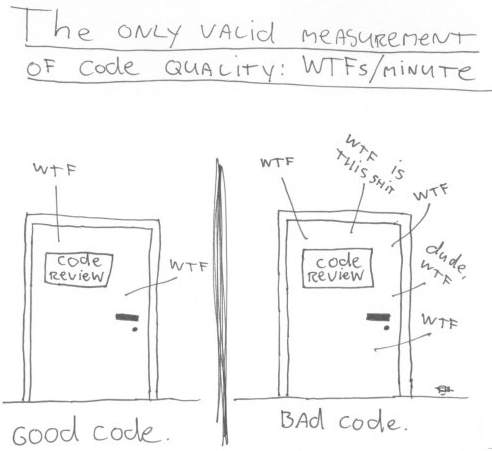
\includegraphics [width=0.5\textwidth] {wtfsm.png}
				\caption{Bewertung der Code-Qualität nach Thom Holwerda \cite{WTFsm}}
				\label{wtfsm}
			\end{figure}
  		\section{Fragestellungen und Vorgehen}
  			Im Folgenden sollen die einzelnen Schritte der konkreten Interpretation der Aufgabenstellung kurz vorgestellt, und daraus resultierende Forschungsfragen abgeleitet werden. In Abbildung~\ref{planning} ist das Vorgehen zur Verdeutlichung des Ablaufs grafisch dargestellt.
  			\begin{enumerate}
				\item Die Grundlage für die Implementierung und Vermessung soll ein in SonarQube zu konfigurierendes Regelwerk darstellen. (Schritt "`Regelwerk"' in Abbildung~\ref{planning})\newline \newline
				\textbf{Nach welchen Programmierregeln sollte die Bewertung hinsichtlich Code-Qualität im Kontext des Softwarepraktikums erfolgen?}
				\item Zusätzlich zu den Metriken soll der Code-Quality-Index als alternative Bewertungsmethode umgesetzt werden. (Schritt "`SWP-Code-Quality-Index"' in Abbildung~\ref{planning})\newline \newline
				\textbf{Inwiefern ist eine Umsetzung des Code-Quality-Index in SonarQube möglich und welche Anpassungen sind notwendig oder sinnvoll?}
				\item Das PlugIn aus dem Großen Beleg soll insbesondere hinsichtlich des Parsers überarbeitet werden. Angedacht ist die Ersetzung des unvollständigen und nur schlecht erweiterbaren "`Eigenbau-Parsers"' durch ExtendJ/Jastadd, um eine langfristige Nutzung des PlugIns zu ermöglichen. (Schritt "`Validierungssystem"' in Abbildung~\ref{planning})\newline \newline
				\textbf{Lässt sich die Stabilität und Wartbarkeit des PlugIns durch die Verwendung von ExtendJ/Jastadd verbessern?}
				\item Mit dem so geschaffenen Messsystem sollen die Programme der letzten zwei Jahrgänge des Softwarepraktikums vermessen werden um die Metrikergebnisse den Bewertungen der Gruppen und deren Selbsteinschätzung gegenüberzustellen. \newline
				(Schritt "`Validierungssystem"' in Abbildung~\ref{planning})\newline \newline
				\textbf{Welche Methoden eignen sich, um die Aussagekraft der Metriken zu evaluieren?}
				\item Die Analyse der Messergebnisse im Vergleich zur Bewertung der Gruppen soll Aufschluss über die Machbarkeit und den konkreten Inhalt des gewünschten (teil-)automatisierten Bewertungssystems geben. (Schritt "`Bewertungssystem"' in Abbildung~\ref{planning})\newline \newline
				\textbf{Welche der umgesetzten Metriken und Bewertungssysteme eignen sich zur teilautomatisierten Bewertung zukünftiger Softwarepraktika?}
				\item Abschließend soll, abhängig von den Antworten auf diese fünf Fragen, das entstandene PlugIn zu einem verwendbaren Bewertungssystem geformt und in die Lehrstuhlinstallation von SonarQube integriert werden. (Schritt "`Bewertungssystem"' in Abbildung~\ref{planning}) 
			\end{enumerate}
  			\begin{figure} [h]
				\centering
				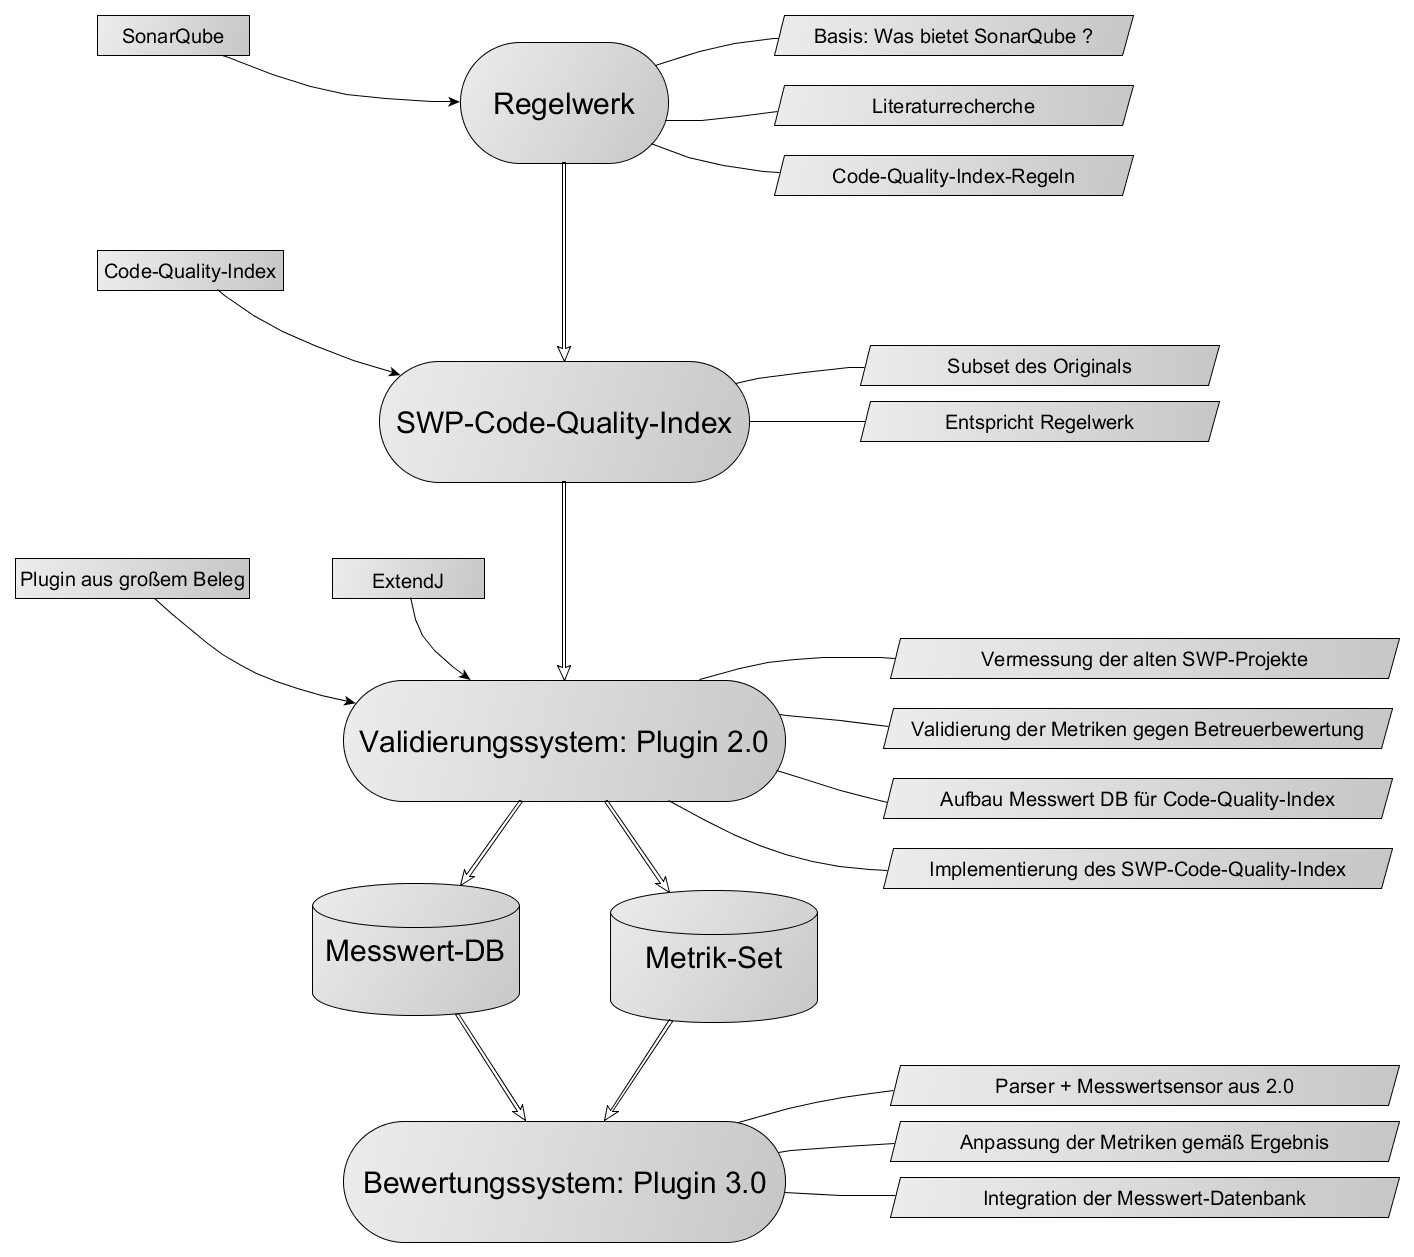
\includegraphics [width=\textwidth] {planning.png}
				\caption{Planung des Vorgehens}
				\label{planning}
			\end{figure}
    
	\chapter{Das Regelwerk}
		Eine der Säulen für ein automatisiertes Bewertungssystem für das Softwarepraktikum ist zwangs-läufig die Festlegung eines geeigneten Regelwerks, dass in SonarQube konfiguriert werden muss und als Basis für diverse Berechnungen zur Beurteilung der abgelieferten Softwarequalität dient. Zum einen fließt die Zahl der Regelverletzungen in mehrere Metriken ein und zum anderen sind diese Regeln, oder Kombinationen mehrerer Regeln gleichzeitig Qualitätsindikatoren des für das Softwarepraktikum angepassten Code-Quality-Index. In diesem Kapitel soll zunächst auf die Notwendigkeit eines Regelwerks eingegangen, einige in der Industrie und Literatur vorgeschlagene Regelwerke vorgestellt und letztlich die getroffene Auswahl begründet und erklärt werden.
		\section{Warum Programmierregeln?}
			Grundsätzlich entsteht die Notwendigkeit für Programmierregeln und "`StyleGuides"' aus zwei für alle Programmiersprachen und Kontexte der Softwareentwicklung gleichen Gegebenheiten: 
			\begin{itemize}
				\item Die Möglichkeiten und Freiheiten die Programmiersprachen bieten gehen weit über das hinaus, was man tun sollte. Für jedes Problem gibt es mehrere Wege zum Ziel von denen viele aber massiv problematisch sind, weil sie beispielsweise sehr fehleranfällig sind, gefährliche Sicherheitslücken aufweisen oder die Performanz der Software negativ beeinflussen. Die Idee hinter vielen Programmierregeln ist daher, ungünstige Konstrukte zu vermeiden ("`Antipattern"') oder bewährte Varianten zu nutzen ("`Best Practices"')
				\item Die meiste Zeit verwendet der Programmierer auf das Lesen von Code, nicht für das eigentliche Schreiben \cite{CleanCode}. Dies gilt selbst für kleine, allein bearbeitete Projekte da auch der selbst geschriebene Code immer wieder gelesen werden muss, um ihn zu erweitern. Der Effekt verstärkt sich bei größeren Projekten, die in Teams bewältigt werden, da nun Code anderer Programmierer gelesen werden muss, um den eigenen Code anbinden zu können. Noch größer ist der Anteil des Code-Lesens, wenn es um die Wartung und Erweiterung von bestehenden Softwaresystemen geht. Daher ist eine gute Lesbarkeit des Codes notwendig, um effizient und effektiv zu programmieren. 
			\end{itemize}
			Beiden Sachverhalten lässt sich am geeignetsten durch ein Regelwerk begegnen, an dass sich alle am Projekt beteiligten Programmierer halten, um so möglichst vielen Fehlerquellen von vorne herein aus dem Weg zu gehen und möglichst gut lesbaren, konsistenten Code zu erhalten, der leicht verstanden und damit erweitert werden kann. Leider gibt es kein allgemeingültiges Regelwerk, das sich für beliebige Projekte anwenden lässt und somit für gute Code-Qualität sorgt. Recht einfach zu erkennen ist, dass zumindest für jede Programmiersprache ein eigenes Regelwerk notwendig ist, da jede Sprache ihre Eigenheiten und speziellen Stolperfallen besitzt. Doch auch innerhalb einer festgelegten Programmiersprache wie im Beispiel des Softwarepraktikums "`Java"' gibt es eine erstaunliche Vielfalt von zum Teil widersprüchlichen Regeln, die auf verschiedenste Art und Weise zu Regelwerken zusammengefasst werden können. Dies lässt sich durch sehr verschiedene Anforderungsprofile der Projekte begründen, aber auch persönliche Vorlieben und Erfahrungen spielen eine große Rolle \cite{JavaQualityAssurance}. Im Folgenden werden Ursachen genannt, die ein allgemeingültiges Regelwerk als nicht sinnvoll, wenn nicht sogar unmöglich erscheinen lassen:
			\begin{labeling}{\textbf{Erfahrung}}
				\item [\textbf{Relevanz}] Manche Regeln sind im Kontext eines speziellen Projekts einfach nicht relevant. Wenn es sich um eine reine Desktop-PC-Anwendung ohne Internetzugriff handelt, sind Regeln die auf sichere Verschlüsselung oder Schutz vor Angriffen abzielen einfach unwichtig. Auch performanzbezogene Regeln spielen an vielen Stellen eine untergeordnete Rolle. 
				\item [\textbf{Zeit}] Programmiersprachen und Techniken verändern sich mit der Zeit. Es ist nur logisch, dass auch die zugehörigen Programmierregeln einer ständigen Überarbeitung und damit Veränderung unterliegen. Die Einführung von "`try-with-resources"' mit Java 1.7 ist ein Beispiel dafür. Gab es zuvor Regeln, die vorgaben geöffnete Resourcen in einem "`finally"'-Block freizugeben \cite{ElementsOfJavaStyle} wird nun von den meisten Autoren empfohlen das neue Sprach-Konstrukt zu verwenden, da so die geöffneten Resourcen automatisch geschlossen werden \cite{JavaCodingGuidelines}.
				\item [\textbf{Erfahrung}] Die Auswahl der Regeln hängt in beträchtlichem Maß von den persönlichen Erfahrungen der verantwortlichen Entwickler ab. Ein Entwickler, der in einem früheren Projekt massive Probleme mit dem "`casten"' von Variablen auf speziellere Datentypen hatte wird eher auf eine Regel bestehen, die genau das verbietet. Jemand dem diese Probleme noch nicht begegnet sind, oder an Programmen gearbeitet hat in dem dies sogar notwendig war, um die gewünschte Funktionalität umzusetzen wird hingegen eher darauf verzichten wollen \cite{JavaQualityAssurance}. Auch sollte das Regelwerk sich gerade im Lehrumfeld am geringen Erfahrungsstand der Studenten oder Schüler orientieren. Ein kleines, leicht zu verstehendes Regelwerk, dass umgesetzt wird, ist hier viel wirksamer, als ein möglichst vollumfängliches, dass die Beteiligten überfordert und eher ignoriert wird \cite{CleanCodeImPraktikum}.
				  \item [\textbf{Vorlieben}] Insbesondere mit Blick auf die Lesbarkeit des Codes spielen die Vorlieben der Entscheider über das Regelwerk eine sehr große Rolle. Es lässt sich nicht festlegen, welcher Stil der beste ist. Wichtig ist allerdings, dass für das Projekt entsprechende Regeln möglichst genau definiert, und konsistent umgesetzt werden. 
				  \item [\textbf{Kontext}] Viele Regeln sind auch vom Projektkontext abhängig. Programme, die in einem Kontext betrieben werden, von dem Menschenleben abhängen, erfordern beispielsweise eine sehr viel höhere Testabdeckung als ein Computerspiel. Eine Software die langfristig betrieben werden soll, erfordert strengere Regeln für Lesbarkeit und Wartbarkeit als ein Prototyp.  
				  \item [\textbf{Ziel}] Neben dem Ziel, ein praktikables Regelwerk für ein konkretes Projekt zu entwerfen, kann das Ziel eines Regelwerks auch sein, einen groben Rahmen für alle Projekte in einem Unternehmen zu schaffen, wodurch die Regelauswahl sehr viel allgemeiner ausfallen wird. Ähnlich ist es, wenn möglichst allgemeingültige Regeln für eine Veröffentlichung in Form eines Buches zusammen getragen werden, oder Studenten die Grundbegriffe von Softwarequalität vermittelt werden sollen.
			\end{labeling}
			Zusammenfassend lässt sich also feststellen, dass für eine hohe Softwarequalität ein für den konkreten Fall zusammengestelltes und angepasstes Regelwerk erforderlich ist, dass darüber hinaus gut und vollständig kommuniziert werden muss, damit es auch Anwendung findet und die gewünschten Effekte bringt \cite{ImproveCodeQuality}.
		\section{Regelwerke} \label{regelwerke}
			Im Rahmen der vorliegenden Arbeit wurde eine Reihe von Regelwerken ausgewertet, um für die Anwendung im Softwarepraktikum eine Schnittmenge zu finden, die möglichst wichtige und weit verbreitete Regeln beinhaltet. Im Folgenden sollen diese kurz vorgestellt und in Bezug auf die Relevanz für das Softwarepraktikum eingeordnet werden. Die Regelbezeichnungen sind den jeweiligen Quellen entnommen und daher zum Teil in englischer Sprache.
			\subsection{Clean Code von Robert Martin} \label{cleancodechapter}
				Robert Martin legt den Fokus seines Buches "`Clean Code"' auf das Erstellen von gut lesbarem Code \cite{CleanCode}. Dies ist im Kontext dieser Arbeit nur ein Teilaspekt von Code-Qualität, aber speziell für die Lehre eine gute Grundlage, um ein Bewusstsein für guten Code zu vermitteln. Dies wird darüber hinaus noch dadurch vereinfacht, dass es in mehreren Sprachen, darunter auch Deutsch, erschienen ist. \newline
				Neben einer ganzen Reihe von Techniken zum Schreiben von sauberem Code gibt der Autor auch viele Hinweise zur Durchführung von Refactorings, also der Transformation von chaotischem Code zu gut Lesbarem. Diese Techniken sind aus seiner Sicht essentiell, da es keinen Softwareentwickler gibt, der im ersten Wurf perfekten Code schreiben kann. Der Code wächst nach und nach, und viele Entscheidungen für die Platzierung von Code-Bausteinen stellen sich im Laufe der Entwicklung als ungünstig heraus. Die Verwendung der Variablen und Methoden ändert sich und die zuvor gewählten Namen passen nicht mehr. Methoden und Klassen wachsen über das sinnvolle Maß hinaus und müssen aufgeteilt werden. So wird es schnell erforderlich, den gerade geschriebenen Code zu überarbeiten, um das gewachsene Chaos zu beseitigen und am Ende guten, sauberen Code abzuliefern. \newline
				Die für das Softwarepraktikum auszuwählenden Regeln sollen allerdings nicht den Prozess des Code Schreibens und der Überarbeitung betrachten, sondern die statische Bewertung des Endergebnisses. Trotzdem finden sich in den von Martin aufgelisteten Regeln neben den nicht maschinell messbaren prozessbezogenen Regeln viele "`Best Practices"' deren Einhaltung sich im Endergebnis messen lassen und damit potenziell Verwendung finden können. In Tabelle~\ref{cleancoderules} finden sich die 25 von insgesamt 66 Regeln aus "`Clean Code"' deren Einhaltung sich vollständig oder zumindest teilweise durch statische Codeanalyse messen lassen. \newline
				Zwei übergeordnete Prinzipien die Martin vorschlägt seien an dieser Stelle explizit erwähnt, da sie in keinem der anderen Regelwerke in dieser Form auftauchen:
				\begin{itemize}
					\item Extreme Kürze der Code-Bausteine, insbesondere Methoden  
					\item Vermeidung von Kommentaren durch selbsterklärenden Code
				\end{itemize}
				\begin{center}
					\tabulinesep=1.5mm
					\begin{longtabu}{|c|c|}
						\hline
  						\textbf{Regel} & \textbf{Kurzbeschreibung}\\
  						\hline
  						Auskommentierter Code & Code sollte nicht auskommentiert werden, Versionsverwaltung \\ & übernimmt Erhaltung von verworfenem Code \\
  						\hline
  						Zu viele Argumente & Maximal 3 Methodenparameter verwenden\\
  						\hline
  						Output-Argumente & Methodenparameter nicht überschreiben und als \\ & "`Ergebnisvariable"' benutzen \\
  						\hline
  						Flag-Argumente & Keine Booleschen Methodenparameter verwenden \\
  						\hline
  						Tote Funktionen & Nicht verwendete Methoden löschen \\
  						\hline
  						Übergangene Sicherungen & IDE-Warnungen, Exceptions und fehlschlagende Tests \\ & nicht Ignorieren \\
  						\hline 
  						Duplizierung & Duplizierte Code-Abschnitte in eigene Methoden auslagern \\ & und wiederverwenden \\
  						\hline
  						Falsche Vererbung & Keine Referenzen auf erbende Klassen in Basisklasse \\
  						\hline
  						Zu viele Informationen & Klassensignaturen (Anzahl öffentlicher Methoden) klein halten \\
  						\hline
  						Toter Code & Nicht verwendeten / erreichbaren Code entfernen \\
  						\hline
  						Vertikale Trennung & Lokale Variablen direkt über erster Verwendung, \\ & private Methoden direkt unter erster Verwendung deklarieren \\
  						\hline
  						Funktionsneid & Nur Variablen der eigenen Klasse manipulieren \\
  						\hline
  						Polymorphismus & Polymorphe Überschreibung von Methoden in Unterklassen \\ anstatt Switch & gegenüber Fallunterscheidung mit "`switch"' bevorzugen \\
  						\hline
  						Konventionen beachten & Im Team festgelegte Code-Konventionen einhalten \\
  						\hline
  						Magic Numbers & Konstante numerische Werte im Code durch sprechend \\ & benannte Konstanten ersetzen \\
  						\hline
  						Bedingungen einkapseln & Nicht triviale Bedingungen für Kontrollfluss-Anweisungen \\ & in eigene Methoden mit sprechendem Namen auslagern \\  
  						\hline
  						Negative Bedingungen & Keine negierten Bedingungen in Kontrollfluss-Anweisungen \\
  						\hline
  						Eine Aufgabe pro Funktion & Methoden sehr kurz halten (4 Anweisungen) \\
  						\hline
  						Grenzbedingungen kapseln & Öfter verwendete In-/Dekremente in Variablen ablegen \\
  						\hline
  						Transitive Navigation & Keine transitiven Methodenaufrufs-Ketten \\
  						\hline
  						Lange Importlisten & Bei Verwendung von mehr als 2 Klassen aus einem "`package"' \\ & "`Wildcard-Import"' benutzen \\
  						\hline
  						Konstanten-Vererbung & Konstanten nicht vererben, sondern statisch importieren \\
  						\hline
  						Enum statt Konstanten & Anstatt "`final static int"' Variablen lieber Enums verwenden \\
  						\hline
  						Kurze Namen & Nur "`Wegwerfvariablen"' (z.B. "`i"' in Schleife) dürfen kurz, \\ & nicht-sprechend benannt werden \\
  						\hline  
  						Unzureichende Tests & Alle Bedingungen durch Tests abdecken \\
  						\hline   
  						\caption{Regeln aus "`Clean Code"' von Robert Martin deren Einhaltung zumindest teilweise durch statische Code-Analyse ermittelbar ist \cite{CleanCode}}
						\label{cleancoderules}
  					\end{longtabu}   
  				\end{center}
			\subsection{Solid Code von Marshall und Bruno}
				Das Buch "`Solid Code"' von Donis Marshall und John Bruno betrachtet umfassend den gesamten Prozess der Softwareentwicklung \cite{SolidCode}. \newline
				Dadurch ist der Aspekt Code-Qualität nur ein verhältnismäßig kleiner Teil des Buches neben Agilen Methoden, Entwurfs- und Design-Techniken, Performanz-Betrachtungen, Debugging und Prozessanalyse. Aus dem Kapitel zur defensiven Programmierung lassen sich allerdings einige, recht allgemeine Regeln ableiten, die, obwohl im Buch "`C\#"' als Programmiersprache verwendet wird, auch für das Softwarepraktikum mit "`Java"' Anwendung finden können. In Tabelle~\ref{solidcoderules} sind die 15 messbaren Regeln der 40 aus dem Kapitel zur Defensiven Programmierung abgeleiteten aufgelistet, die nicht als "`C\#"'-spezifisch eingestuft werden.
				\begin{center}
					\tabulinesep=1.5mm
					\begin{longtabu}{|c|c|}
						\hline
  						\textbf{Regel} & \textbf{Kurzbeschreibung}\\
  						\hline
  						Softwaretest & Testabdeckung der Anweisungen von mindestens 90\% \\ 
  						\hline   
  						Namenskonventionen & Namenskonventionen für Team festlegen und umsetzen \\
  						\hline
  						Dokumentationskommentare & Mindestens alle öffentlichen Code-Elemente mit \\ & Dokumentationskommentaren (z.B. Javadoc) versehen \\
  						\hline
  						Klassen & Keine öffentlichen Variablen in Klassen verwenden \\
  						\hline
  						Zugriffsmodifizierer & Klassen und "`Class-Members"' so restriktiv wie möglich \\ & deklarieren (Sichtbarkeit, Modifizierbarkeit, ...) \\
  						\hline
  						Rückgabewerte & Rückgabewerte von Methoden immer überprüfen \\
  						\hline
  						Literale & Anstatt Literalen im Code sprechend benannte \\ &  Konstanten verwenden \\
  						\hline
  						Default Case & Jede "`switch"'-Anweisung sollte einen "`default"'-Case haben \\
  						\hline
  						Allgemeine Exceptions & Allgemeine "`Exceptions"' sollten nicht abgefangen werden \\
  						\hline
  						Fallunterscheidung & In "`catch"'-Blöcken sollte keine Fallunterscheidung \\ für Exceptions & Anhand des "`Exception"'-Typs erfolgen \\
  						\hline
  						Duplizierung & Duplizierte Code-Abschnitte in eigene Methoden auslagern \\ & und wiederverwenden \\
  						\hline
  						Schleifentypen & "`for"'-Schleifen gegenüber "`while"'-Schleifen bevorzugen \\
  						\hline
  						Freiwillige Blöcke & Optionale geschweifte Klammern immer verwenden \\ & (in If-/While-/For-Anweisungen) \\
  						\hline
  						Groß-/Kleinschreibung & Bezeichner dürfen nicht nur durch Groß-/Klein- \\ & Schreibung unterschieden werden \\
  						\hline
  						Switchvariable & Als "`switch"'-Variable nur Enums verwenden \\
  						\hline
  						\caption{Regeln aus dem Kapitel "`Defensive Programmierung"' im Buch "`Solid Code"' von Marshall und Bruno die auf Java übertragbar sind und deren Einhaltung zumindest teilweise durch statische Code-Analyse ermittelbar ist \cite{SolidCode}}
						\label{solidcoderules}
  					\end{longtabu}   
  				\end{center}
			\subsection{Elements of Java Style von Vermeulen et al.}
				Das älteste der ausgewerteten Regelwerke ist das Buch "`The Elements of Java Style"' von Allan Vermeulen et al. \cite{ElementsOfJavaStyle} aus dem Jahr 2000. Dabei handelt es sich vorrangig um eine Unternehmensrichtline für das Schreiben von Java-Code bei "`Rogue Wave\textsuperscript{\textregistered} Software"', angereichert mit Regeln weiterer, unternehmensfremder Autoren. Trotz des Alters dieses Regelwerks sind nur sehr wenige Regeln als veraltet zu betrachten, wie beispielsweise das Freigeben von Ressourcen mittels "`finally"'-Block anstatt dem mittlerweile üblichen "`try-with-resources"' oder die händische Kapselung von Enumerationen in Klassen. \newline
				Das Buch konzentriert sich ausschließlich auf das Schreiben von möglichst verständlichem, wartbaren Java-Code. Trotzdem ist die Einhaltung vieler der angeführten Regeln nicht durch statische Codeanalyse messbar. In Tabelle~\ref{elementsrules} sind daher wiederum nur die Regeln aufgeführt die diese Bedingung erfüllen und darüber hinaus nicht veraltet sind. Dies sind 39 der 108 im Buch aufgeführten Regeln. \newline
				Allerdings kommt hier die Betrachtung des Software-Lebenszyklus hinzu, der im Rahmen des Softwarepraktikums irrelevant ist. So gibt es einige Regeln die sich auf die Erweiterung und Wartung von Software über mehrere Versionen hinweg beziehen. Darüber hinaus fällt auf, dass sehr großen Wert auf ausführliche Kommentierung des Codes gelegt wird, obwohl selbsterklärender Code als vorrangiges Ziel genannt wird, was laut anderen Autoren eine ausführliche Kommentierung überflüssig macht und sogar als potenzielles Problem eingestuft wird, da die Kommentare mit gepflegt werden müssen und veraltete und damit falsche Kommentare schlimmer sind als gar keine, da sie in die Irre führen können \cite{CleanCode}.
				\begin{center}
					\tabulinesep=1.5mm
					\begin{longtabu}{|c|c|}
						\hline
  						\textbf{Regel} & \textbf{Kurzbeschreibung}\\
  						\hline
  						Indent nested code & Konsistente Einrückung \\
  						\hline
  						Long lines & Maximale Zeilenlänge festlegen und einhalten \\
  						\hline
  						White space & Leerzeichen vor/nach Klammern und Operatoren, Leerzeilen \\ & zwischen Klassen, "`Class-Members"' und logischen Abschnitten \\
  						\hline 
  						No tabs & Nur Leerzeichen, keine Tabs verwenden \\
  						\hline
  						Long names & Keine zu langen Bezeichner verwenden \\
  						\hline
  						Names different & Bezeichner dürfen nicht nur durch Groß-/Klein- \\ in case & Schreibung unterschieden werden \\
  						\hline
  						Package name & Einzelnes, klein geschriebenes Wort für "`package"'-Namen \\
  						\hline
  						Class Name & Klassennamen in "`Upper CamelCase"' \\  							\hline
  						Method Name & Methodennamen in "`Lower CamelCase"' \\ 
  						\hline
  						Java Bean conventions & "`JavaBeans"' Namenskonventionen für \\ & "`getter"' und "`setter"' verwenden \\
  						\hline
  						Variable names & Variablennamen in "`Lower CamelCase"' \\ 
  						\hline
  						Qualify field variables & Klassenvariablen immer mit "`this"' referenzieren \\
  						\hline
  						Assign parameters & Methoden-/Konstruktor-Parameter die Klassenvariablen \\ to fields & zugewiesen werden, sollten den gleichen Namen haben \\
  						\hline
  						Constant Name & Für Konstantennamen nur Großbuchstaben verwenden \\
  						\hline
  						Javadoc & Javadoc für alle Klassen, Interfaces, Methoden, Klassenvariablen \\
  						\hline
  						Package documentation & Für alle "`packages"' Kommentardatei schreiben \\
  						\hline
  						Javadoc style & Alle Javadoc-Kommentare nach SUN-Konventionen formatieren \\
  						\hline
  						Javadoc code tag & Bezeichner, Schlüsselwörter und Konstanten in \\ & Javadoc-Kommentaren mit "`code"'-Tag versehen \\
  						\hline 
  						Method Javadoc & Methodensignatur vollständig in Javadoc beschreiben \\
  						\hline
  						End line comments & Keine Kommentare an Zeilenende (außer Variablendeklaration) \\
  						\hline
  						Variable comment & Deklaration lokaler Variablen am Zeilenende kommentieren \\
  						\hline
  						Nested block comment & Bei tiefer Verschachtelung schließende Klammer \\ & mit Kommentar versehen \\
  						\hline
  						Fall through comment & Wenn "`switch-case"' nicht durch "`break"'-Anweisung \\ & abgeschlossen wird, durch "`fall-through"' Kommentar abschließen \\
  						\hline
  						Empty block comment & Leere Blöcke kommentieren \\
  						\hline
  						Small classes/methods & Klassen und Methoden möglichst klein halten \\
  						\hline
  						Private fields & Alle Klassenvariablen als privat deklarieren \\
  						\hline
  						Polymorphism & Polymorphe Methoden-Implementation anstatt \\ & "`instanceof"' verwenden \\
  						\hline
  						Duplicated blocks & Duplizierte Code-Abschnitte in eigene Methoden auslagern \\ & und wiederverwenden \\
  						\hline
  						Block statements & Optionale geschweifte Klammern immer verwenden \\ & (in If-/While-/For-Anweisungen) \\
  						\hline
  						Last case & Der letzte "`case"' in einem "`switch"' muss durch \\ & "`break"'-Anweisungen abgeschlossen werden \\
  						\hline
  						Compare Objects & Objekte mittels "`equals"'-Methode vergleichen \\
  						\hline
  						Construction final & In Konstruktoren nur Methoden aufrufen \\ & die als "`final"' deklariert sind \\
  						\hline
  						Nested constructors & Allgemeine Konstruktoren in speziellen aufrufen \\
  						\hline
  						Runtime exceptions & "`Runtime-Exceptions"' nicht abfangen \\
  						\hline
  						Exception forwarding & Beim weiterleiten von "`Exceptions"' keine \\ & Informationen entfernen, lediglich anreichern \\
  						\hline   
  						Empty catch & Keine leeren "`catch"'-Blöcke verwenden \\
  						\hline
  						Object instances & Objektinstanzen erst erzeugen, wenn sie gebraucht werden \\
  						\hline
  						Unnecessary objects & Keine unnötigen Objektinstanzen anlegen \\
  						\hline
  						Object factory & "'Factory"' zur Verwaltung von wiederverwendbaren \\ & Objektinstanzen nutzen \\
  						\hline
  						
  						\caption{Regeln aus "`The Elements of Java Style"' von Vermeulen et Al. die noch Gültigkeit haben und deren Einhaltung zumindest teilweise durch statische Code-Analyse ermittelbar ist \cite{ElementsOfJavaStyle}}
						\label{elementsrules}
  					\end{longtabu}   
  				\end{center}
			\subsection{Code-Quality-Management von Simon et al.} \label{cqirules}
				Im Buch "`Code-Quality-Management"' beschreiben Frank Simon et Al. kein Regelwerk im eigentlichen Sinne \cite{CodeQualityManagement}. Stattdessen werden 52 Qualitätsindikatoren aufgeführt, die jeweils aus Folgenden Bestandteilen zusammengesetzt werden:
				\begin{itemize}
					\item Ein Problemmuster, dass im Wesentlichen einer Programmierregel entspricht.
					\item Vier Schwellwertstufen bezüglich der Häufigkeit des Problemmusters. 
					\item Gewichtete Zuordnung zu einem oder mehreren Qualitätsmerkmalen.
					\item Beurteilung bezüglich Kosten und Unmittelbarkeit der Wirkung einer Behebung. 
				\end{itemize} 
				Diese Indikatoren werden benutzt um das zu untersuchende Programm, als stark vereinfachte Qualitätsbeurteilung, einem Benchmark-Level zuzuordnen. Dieses Verfahren wird als Code-Quality-Index bezeichnet und ist eine Alternative zur Bewertung der Code-Qualität im Vergleich zu den von Harry Sneed und anderen Autoren vorgeschlagenen Metriken \cite{SoftwareInZahlen}. Der Code-Quality-Index wurde bereits im dieser Arbeit vorangegangenem Großen Beleg untersucht \cite{grosserBeleg} und soll in abgewandelter Form im zu erweiternden SonarQube-Plugin für das Bewertungssystem umgesetzt werden (siehe Kapitel \ref{indexchapter}). Als Grundlage wurden für das Regelwerk daher alle Problemmuster der 52 Indikatoren als Regeln mit aufgenommen, dargestellt in Tabelle~\ref{indexrules}.  
				\begin{center}
					\tabulinesep=1.5mm
					\begin{longtabu}{|c|c|}
						\hline
  						\textbf{Regel} & \textbf{Kurzbeschreibung}\\
  						\hline
						Allgemeine Parameter & Casting von Methodenparametern vermeiden \\
						\hline
						Attributüberdeckung & Verwenden gleicher Variablennamen in Unterklassen vermeiden \\
						\hline
						Ausgeschlagenes Erbe & Methodenimplementierung von Oberklasse sollte von \\ - Implementierung & Mehrheit der Unterklassen nicht überschrieben werden \\
						\hline
						Ausgeschlagenes Erbe & Reduktion von Sichtbarkeiten in Unterklassen und \\ - Schnittstelle & Leer-Implementierung von Schnittstellen vermeiden \\
						\hline
						Datenkapselaufbruch & Keine öffentlichen Klassenvariablen verwenden \\
						\hline
						Duplizierter Code & Duplizierten Code vermeiden (>40 aufeinander folgende Zeilen) \\
						\hline
						Falsche Namenslänge & Bezeichner zwischen 2 und 50 Zeichen verwenden \\
						\hline
						Generationskonflikt & Erbende Klassen sollten höchstens die Hälfte der Oberklasse \\ & überschreiben ohne Oberklassenimplementierung zu nutzen \\
						\hline
						Gottdatei & Dateien sollten weniger als 2000 Zeilen enthalten \\
						\hline
						Gottklasse (Attribut) & Klassen sollten weniger als 50 Instanzvariablen deklarieren \\
						\hline
						Gottklasse (Methode) & Eine Klasse sollte weniger als 50 Methoden deklarieren \\
						\hline
						Gottmethode & Eine Methode sollte weniger als 200 Zeilen haben \\
						\hline
						Gottpaket & Ein "`package"' sollten höchstens 50 Klassen enthalten \\
						\hline
						Halbherzige Operationen & Klassen die equals() implementieren sollten auch \\ &  hashCode() implementieren \\
						\hline
						Heimliche Verwandschaft & Öffentliche Methoden einer Oberklasse sollten nicht nur \\ & von erbenden Klassen verwendet werden \\
						\hline
						Identitätsspaltung & Klassen sollten nicht den gleichen Namen haben \\ & oder sich nur durch Groß-/Kleinschreibung unterscheiden \\
						\hline
						Importchaos & Imports nicht doppelt, aus gleichem package, \\ & von java.lang oder als "`Wildcard"' \\
						\hline
						Importlüge & Unbenutzte Imports entfernen \\
						\hline
						Informelle & Öffentliche Methoden müssen formal kommentiert werden \\ Dokumentation & \\
						\hline
						Interface-Bypass & Implementation eines Methodeninterfaces sollten nicht \\ & direkt genutzt werden sondern über abstraktes Interface \\
						\hline
						Klässchen & Öffentliche Klassen sollten mindestens drei \\ & Methoden oder Klassenvariablen haben \\
						\hline
						Klasseninzest & Klassen dürfen keine Referenzen auf erbende Klassen haben \\
						\hline
						Konstantenregen & Namen von Konstanten sollten nur \\ &  einmal im System vorkommen \\
						\hline
						Labyrinthmethode & Die McCabe-Komplexität einer Methode sollte nicht >10 sein \\
						\hline
						Lange Parameterliste & Methoden sollten nicht mehr als 7 Parameter haben \\
						\hline
						Maskierende Datei & Dateiname sollte in enthaltener Klasse vollständig vorkommen \\
						\hline
						Nachlässige & (Dateizeilen - 2 * Kommentarzeilen) möglichst klein \\ Kommentierung & (Eine Kommentarzeile je Codezeile) \\
						\hline
						Namensfehler & Standard-Java-Namenskonventionen einhalten \\
						\hline
						Objektplacebo (Attribut) & Statische Attribute sollten nur statisch referenziert werden \\
						\hline
						Objectplacebo (Methode) & Statische Methoden sollten nur statisch referenziert werden \\
						\hline
						Paketchen & Pakete sollten mindestens drei öffentliche Klassen enthalten \\
						\hline
						Pakethierarchieaufbruch & Oberklassen sollten nicht in untergeordneten Paketen liegen, \\ & wenn erbende Klassen in übergeordneten Paketen liegen \\
						\hline
						Polymorphieplacebo & Statische Methoden der Oberklasse sollten nicht in \\ & erbenden Klassen überdeckt werden \\
						\hline
						Potenzielle Privatsphäre & Sichtbarkeiten von Variablen sollten so weit \\ (Attribut) & wie möglich eingeschränkt werden \\
\hline
						Potenzielle Privatsphäre & Methoden sollten nur protected deklariert werden wenn \\ (Methode) & sie eine Methode überschreiben oder überschrieben werden \\
						\hline
						Pränatale Kommunikation & In Konstruktoren nur "`finale"' Methoden aufrufen \\
						\hline
						Risikocode & "`Break"' in jeder Case-Anweisungen, Default-Case in \\ & jeder Switch-Anweisung und keine leeren Catch-Anweisungen \\
						\hline
						Signaturähnliche Klassen & Höchstens 50\% identische Methodensignaturen zweier Klassen \\
						\hline
						Simulierte Polymorphie & Objekte sollten in einer Methode nicht auf mehrere \\ & Objekttypen überprüft werden (durch "`instanceof"') \\
						\hline
						Späte Abstraktion & Abstrakte Klassen sollten nicht von Nicht-Abstrakten erben \\
						\hline
						Tote Attribute & Ungenutzte private Variablen sollten entfernt werden \\
						\hline
						Tote Implementierung & Anweisungen die nie ausgeführt werden entfernen \\
						\hline
						Tote Methoden & Ungenutzte private Methoden sollten entfernt werden \\
						\hline
						Überbuchte Datei & Pro Datei nur eine übergeordnete öffentliche Klasse \\
						\hline
						Unfertiger Code & "`ToDo"' / "`FixMe"' / "`Hack"' -  sollte behoben werden \\
						\hline
						Unvollständige Vererbung & Eine nicht-statische Variable sollte nicht in mehr als 50\% \\ (Attribut) & der erbenden Klassen einer Oberklasse vorkommen \\
						\hline
						Unvollständige Vererbung & Eine Methodensignatur sollte nicht in mehr als 50\% \\ (Methode) & der erbenden Klassen einer Oberklasse vorkommen \\
						\hline
						Verbotene Dateiliebe & Zwei Dateien sollten nicht gegenseitig voneinander Abhängen \\
						\hline
						Verbotene Klassenliebe & Zwei nicht durch Vererbung zusammenhängende Klassen \\ & sollten nicht gegenseitig voneinander abhängen \\
						\hline
						Verbotene Methodenliebe & Zwei Methoden sollten sich nicht gegenseitig aufrufen \\
						\hline
						Verbotene Paketliebe & "`packages"' sollten nicht gegenseitig voneinander abhängen \\
						\hline
						Versteckte Konstantheit & Klassenvariablen die nach initialisierung nicht verändert \\ & werden sollten als "`final"' deklariert werden \\
  						\hline
  						\caption{Regeln aus "`Code-Quality-Management"' von Simon et Al. \cite{CodeQualityManagement}}
						\label{indexrules}
  					\end{longtabu}   
  				\end{center}
			\subsection{Java Coding Guidelines von Long et al.}
				Das Buch "`Java Coding Guidelines"' von Fred long et Al. konzentriert sich vornehmlich auf die Entwicklung sicherer und zuverlässiger Web-Anwendungen mit Java \cite{JavaCodingGuidelines}. Es basiert auf dem Buch "`The CERT Oracle Secure Coding Standard for Java"' von den gleichen Autoren \cite{SecureCodingStandard} und ist im Rahmen dieser Arbeit nur bedingt relevant, da eine ganze Reihe der vorgeschlagenen Regeln nicht die Java-Programmierung selbst betrachten sondern auf Sicherheitsaspekte abzielen, wie die Speicherung von Passwörtern und Ähnlichem. Trotzdem verbleiben 21 der 75 Regeln, die grundsätzliche Aspekte beinhalten und daher auch für das Softwarepraktikum betrachtet werden sollen (siehe Tabelle~\ref{guidelinesrules}). Diese Regeln sind ebenso für die Sicherheit und Zuverlässigkeit einer Web-Anwendung relevant, als auch unter dem allgemeineren Blickwinkel der Software-Qualität interessant. 
				\begin{center}
					\tabulinesep=1.5mm
					\begin{longtabu}{|c|c|}
						\hline
  						\textbf{Regel} & \textbf{Kurzbeschreibung}\\
  						\hline
  						Variable scope & Geltungsbereich von Variablen so klein wie möglich halten\\
						\hline
						Accessibility & Sichtbarkeit aller Konstrukte so gering wie möglich halten\\
						\hline
						Cyclic packages & Packages sollten nicht gegenseitig voneinander abhängen \\
						\hline
						Exception types & Möglichst eigene Exception-Typen verwenden \\
						\hline
						Garbage Collection & Möglichst kleine Objekte und \\ & keine expliziten Aufrufe des Garbage Collectors verwenden \\
						\hline
						Shadow identifiers & Bezeichner sollten nicht überdeckt werden \\
						\hline
						Declaration & Nur eine Variable pro Deklarationsanweisung \\
						\hline
						Constants & Literale als konstante Klassenvariablen deklarieren \\
						\hline
						Return empty & Leere Collections zurückgeben anstatt null \\
						\hline
						Try-with-resources & Wenn möglich try-with-resources verwenden \\
						\hline
						Visually misleading & Verwechselbare Zeichen nicht als alleinige Bezeichner oder \\ & einzigen Unterschied zwischen Bezeichnern verwenden \\
						\hline
						Overload variable & Methoden mit variablen Parameterlisten nicht überladen \\
						\hline
						Assignments & In Bedingungen keine Wertzuweisung vornehmen \\
						\hline
						Optional braces & Für alle if, for und while Anweisungen Klammern setzen \\
						\hline
						Empty conditionals & Keine leeren Kontrollflussanweisungen verwenden \\ & (nur Semikolon direkt hinter der Bedingung) \\
						\hline
						Break case & Case-Anweisungen immer mit break abschließen \\
						\hline
						Loop counters & Für Schleifen keine unereichbaren oder überspringbaren \\ & Abbruchbedingungen definieren \\
						\hline
						Clone & Alle clone() Methoden müssen super.clone() aufrufen \\
						\hline
						Unused & Ungenutzten Code, sowie Code ohne Effekte entfernen \\
						\hline
						Confusing overload & Überladene Methoden nicht nur in Reihenfolge der \\ & Parametertypen unterscheiden \\
						\hline
						Object equality & Objekte mit equals vergleichen \\
  						\hline
  						\caption{Regeln aus "`Java Coding Guidelines"' sich auf grundsätzliche Java-Programmierung beziehen und deren Einhaltung zumindest Teilweise durch statische Code-Analyse ermittelbar ist \cite{JavaCodingGuidelines}}
						\label{guidelinesrules}
  					\end{longtabu}   
  				\end{center}
			\subsection{Google Java Style Guide}
				Der "`Google Java Style Guide"' stellt eine vollständige Definition der von Google angesetzten Programmierregeln für die Sprache Java dar und wird bei allen für Google entwickelten Projekte in dieser Sprache angewendet  \cite{GoogleStyleGuide}. Ähnliche Regelwerke gibt es bei Google auch für viele andere gängige Programmiersprachen. Dieses Online verfügbare Dokument wird fortlaufend überarbeitet und weiterentwickelt. Im Rahmen dieser Arbeit wird der Stand von März 2017 betrachtet. Ein Anspruch des Regelwerks ist es, dass alle Regeln so klar sind, dass sie bereits in einer Entwicklungsumgebung erzwungen werden können. Regeln und Hinweise die Interpretationsspielraum lassen und subjektiv vom Betrachter abhängen wie zum Beispiel, das Vergeben sprechender Bezeichner, sind daher nicht aufgeführt. \newline
				Da es sich um eine Unternehmensrichtlinie handelt, sind die Regeln auch auf eine spezielle Art der Formatierung festgelegt und nicht auf die allgemeine Forderung nach Konsistenz beschränkt. Für das Softwarepraktikum muss nicht zwangsläufig die gleiche Formatierung gewählt, aber der Style Guide liefert eine gute Zusammenfassung, an welchen Stellen die Formatierung einheitlich sein sollte und was in der industriellen Praxis üblich ist. Außerdem ist es mit Abstand das aktuellste der ausgewerteten Regelwerke. Die 55 extrahierten Regeln sind in Tabelle~\ref{googlerules} aufgelistet. Diese sind aufgrund der anderen Herangehensweise deutlich detaillierter als in den zuvor genannten Büchern.
				\begin{center}
					\tabulinesep=1.5mm
					\begin{longtabu}{|c|c|}
						\hline
  						\textbf{Regel} & \textbf{Kurzbeschreibung}\\
  						\hline
  												\hline
						Filename & Dateiname = Top-Level-Klassenname + Endung .java \\
						\hline
						File encoding & Datei-Encoding in UTF-8 \\
						\hline
						Whitespace & Nur Standardleerzeichen verwenden (keine Tabs) \\
						\hline
						Escape sequences & Spezielle Escape-Sequenzen anstatt Unicode-Repräsentation \\
						\hline
						Non-ASCII characters & Nicht-ASCII Zeichen nur innerhalb von String Literalen \\
						\hline
						Source file structure & Jede Datei soll folgende Struktur haben: \\ & Lizenz-Info + Package-Anweisung + Import-Anweisungen \\ &  + EINE Top-Level-Klasse \\
						\hline
						License information & Wenn benötigt am Dateianfang, als Block-Kommentar \\
						\hline
						Package Statement & Package-Anweisung immer in eine Zeile schreiben \\
						\hline
						No wildcard imports & Keine wildcard imports verwenden \\
						\hline
						No line-wrapping & Import-Anweisungen immer in eine Zeile schreiben \\
						\hline
						Ordering and spacing & Erst alle statischen imports als Block, dann alle anderen. \\ & Die Blöcke getrennt und alphabetisch sortiert \\
						\hline
						No static import& Statische Klassen nicht mit statischem import einbinden \\
						\hline
						One top-level class& Genau eine Top-Level Klasse je Datei \\
						\hline
						Class contents & Logische Ordnung in Klassen, \\ & Überladene  Methoden direkt aufeinanderfolgend \\
						\hline
						Optional Braces & Alle optionalen geschweiften Klammern setzen \\
						\hline
						Nonempty blocks & Nichtleere Blöcke mit öffnender Klammer an Zeilenende und \\ & schließender Klammer in eigener Zeile schreiben \\
						\hline
						Empty blocks & In Multi-Block-Anweisungen leere Blöcke mit Zeilenumbruch \\
						\hline
						Block indentation & Als Einrückung für Blockinhalt 2 Leerzeichen verwenden \\
						\hline
						Statements per line & Nur eine Anweisung pro Zeile schreiben \\
						\hline
						Column limit & Maximale Zeilenlänge = 100 Zeichen \\
						\hline
						Where to break & Anweisungen in mehreren Zeilen vermeiden \\
						\hline
						Indent continuation & Einrückung bei Zeilenumbruch innerhalb von Anweisung \\ & mindestens 4 Leerzeichen einrücken \\
						\hline
						Vertical whitespace & Leerzeilen zwischen "`Class-Members"' außer Variablen \\
						\hline
						Horizontal whitespace & Genau definiert, siehe Style-Guide  \\
						\hline
						Horizontal alignment & Horizontale Ausrichtung nicht verwenden \\
						\hline
						Grouping parentheses & Klammern zur Gruppierung komplexer Operationen verwenden \\
						\hline
						Enum classes & Enumwerte in einer Zeile, oder mit Zeilenumbruch nach Komma \\
						\hline
						Variable declarations & Nur eine Variable je Anweisung deklarieren \\
						\hline
						Arrays & Eckige Klammern immer am Typ und nicht am variablennamen \\
						\hline
						Switch Statements & Jedes Switch muss default case haben  \\
						\hline
						Annotations & Annotationen an Klassen, Methoden oder Konstruktoren \\ & hinter Javadoc, je eine Annotation pro Zeile \\
						\hline
						Comments & Kommentare genauso einrücken wie umgebender Code \\
						\hline
						Modifiers & Modifiers in fester Reihenfolge \\
						\hline
						Numeric Literals & Literale vom Typ long mit groß geschriebenem L \\
						\hline
						Zeichensatz & Nur ASCII Buchstaben und Zahlen in Namen verwenden \\
						\hline
						Package names & Package Namen komplett klein \\
						\hline
						Class names & Klassennamen in Upper CamelCase \\
						\hline
						Method names & Methodennamen in Lower CamelCase \\
						\hline
						Constant names & Konstantennamen komplett groß \\
						\hline
						Field names & Globale Variablennamen in Lower CamelCase \\
						\hline
						Parameter names & Parameternamen in Lower CamelCase \\
						\hline
						Variable names & Lokale Variablennamen in Lower CamelCase \\
						\hline
						Type names & Typvariablen sind einzelner großer Buchstabe \\
						\hline
						Camel case & Abkürzungen in CamelCase nur mit erstem Buchstaben groß \\
						\hline
						@Override & Überschreibende Methoden mit @Override markieren \\
						\hline
						Caught exceptions & Keine leeren Catch-Anweisungen, außer in Tests \\
						\hline
						Static Members & Statische Methoden und Variablen nur über Klassennamen \\ & referenzieren, nicht über Instanzen \\
						\hline
						Finalizers & finalize() Methode nicht überschreiben \\
						\hline
						General form & Start und Ende von Javadoc Kommentar in eigene Zeile \\
						\hline
						Paragraphs & Zwischen Absätzen in Javadoc eine Leerzeile nur mit * \\
						\hline
						Block tags & Tags in Javadoc-Kommentaren in fester Reihenfolge \\
						\hline
						Summary fragmnet & Erste Zeile eines Javadoc Kommentars ist Zusammenfassung \\ & ohne Subject abgeschlossen mit einem . \\
						\hline
						Where Javadoc & Javadoc an öffentlichen Klassen und "Class-Members" \\
						\hline
						Self-explanatory & Kein Javadoc an trivialen Methoden (getter / setter) \\
						\hline
						Overrides & Überschriebene Methoden brauchen kein Javadoc \\
						\hline
  						\caption{Regeln des "`Google Java Style Guide"'  \cite{GoogleStyleGuide}}
						\label{googlerules}
  					\end{longtabu}   
  				\end{center}
			\subsection{SoftAudit von Harry Sneed}
				Harry Sneed verwendet in seinem Software-Analyse-Werkzeug "`SoftAudit"' 80 Regeln um Fehlerberichte von Java-Programmen zu erstellen. Darüber hinaus geht die Anzahl der gefundenen Regelverletzungen in mehreren Metriken die auch im vorangegangenen Großen Beleg umgesetzt wurden \cite{grosserBeleg} mit in die Berechnung ein. Da es sich hierbei allerdings um eine Anwendung und keine Literatur-Quelle handelt sind die Regeln nicht detailliert erklärt \cite{SoftAuditDoku}. Im Gegensatz zu allen anderen Quellen nimmt Harry Sneed allerdings eine Abstufung der Regeln nach Fehlergewichtung vor. Er unterteilt die verwendeten Regeln in folgende vier Klassen:
				\begin{itemize}
					\item "`Security"' - Sicherheitskritisch 
					\item "`Deficiency"' - Schwerwiegendes Problem
					\item "`Problem"' - Möglicher Fehler
					\item "`Warning"' - Hinweise auf schlechten Stil
				\end{itemize}
				Diese finden sich in ähnlicher Form auch in der Zielplattform SonarQube wieder und bieten einen Anhaltspunkt für eine mögliche Klassifizierung der letztendlich ausgewählten Regeln. In Tabelle~\ref{softauditrules} sind die Regeln in der Originalformulierung zusammen mit der Einstufung aufgeführt.
				\begin{center}
					\tabulinesep=1.5mm
					\begin{longtabu}{|c|c|}
						\hline
  						\textbf{Einstufung} & \textbf{Regel}\\
  						\hline
						Problem & IO Operations must be contained be in a try block \\
						\hline
						Problem & Two Dimensional Arrays conflict with 1. Normal Form \\
						\hline
						Problem & Data Redefinitions conflict with 2. Normal Form \\
						\hline
						Problem & Data Casting should be avoided \\
						\hline
						Security & Constructor Methods should not be duplicated \\
						\hline
						Problem & Synchronization should be avoided \\
						\hline
						Problem & Method Invocation with array of objects should be in try block \\
						\hline
						Security & Return Value is not controlled after method invocation \\
						\hline
						Problem & Conditions should not contain an Assignment \\
						\hline
						Problem & Break is missing in switch Statement \\
						\hline
						Problem & Default is missing in switch Statement \\
						\hline
						Problem & Control logic exceeds maximum Nesting Level \\
						\hline
						Problem & More than one Statement on a Line \\
						\hline
						Security & Class Variables should never be declared public \\
						\hline
						Problem & instanceof should not be used \\
						\hline
						Problem & External Method Invocation should have a Class Reference \\
						\hline
						Security & Return Values should be checked \\
						\hline
						Security & Derived class is not declared as final \\
						\hline
						Problem & Class should not contain labels \\
						\hline
						Problem & Class attribute names should be qualified \\
						\hline
						Problem & equals should be used to compare objects \\
						\hline
						Problem & Interface definition should be in a separate source file \\
						\hline
						Security & Input Parameters of a Public Method should be checked \\
						\hline
						Problem & Returning a function may cause an endless loop \\
						\hline
						Problem & Number of catches does not match number of tries \\
						\hline
						Deficiency & Source module exceeds maximum size limit \\
						\hline
						Deficiency & Source module has more than maximum allowed Statements \\
						\hline
						Deficiency & Source module has more than maximum allowed Imports \\
						\hline
						Deficiency & Source module has more than maximum allowed Variables \\
						\hline
						Deficiency & Source module has more than maximum allowed Interfaces \\
						\hline
						Deficiency & Source module has more than maximum allowed Classes \\
						\hline
						Deficiency & Source module has more than maximum allowed Methods \\
						\hline
						Deficiency & Class exceeds maximum size limit \\
						\hline
						Deficiency & Method exceeds maximum size limit \\
						\hline
						Deficiency & Method has more than maximum allowed Parameters \\
						\hline
						Deficiency & Module references too many foreign Methods \\
						\hline
						Deficiency & Package should have a documentation header \\
						\hline
						Deficiency & Interface should have a documentation header \\
						\hline
						Deficiency & Class should have a documentation header \\
						\hline
						Deficiency & Method should have a documentation header \\
						\hline
						Deficiency & Compound Condition has more than two condition clauses \\
						\hline
						Deficiency & ? Operation should not be used in Expressions \\
						\hline
						Deficiency & Documentation header should include a code tag \\
						\hline
						Deficiency & Methods without Return value should be void \\
						\hline
						Deficiency & String Vectors should be avoided \\
						\hline
						Deficiency & Constants in procedural statements are forbidden \\
						\hline
						Deficiency & Literals in procedural statements are forbidden \\
						\hline
						Security & Embedded SQL functions should be avoided \\
						\hline
						Security & SQL Statement strings in code are vulnerable \\
						\hline
						Warning & Imports should proceed all other statements \\
						\hline
						Warning & Database Accesses are restricted to access classes \\
						\hline
						Warning & Nested Code should be indented by at least two columns \\
						\hline
						Warning & Code Line should not exceed maximum length of 120 Characters \\
						\hline
						Warning & Data Declaration should be followed by a Comment \\
						\hline
						Warning & Structure and union declarations should be proceeded by a comment \\
						\hline
						Warning & End Bracket should be followed by a Comment \\
						\hline
						Warning & Control Command should be on a separate line \\
						\hline
						Warning & Numeric constants should not start with a decimal point \\
						\hline
						Warning & Open Block Bracket should be on a separate line \\
						\hline
						Warning & Close Block Bracket should be on a separate line \\
						\hline
						Warning & Left Parenthesis should be proceeded by a space \\
						\hline
						Warning & Right Parenthesis should be followed by a space or Semicolon \\
						\hline
						Warning & Arithmetic Operator should be delimited by spaces \\
						\hline
						Warning & Logical Operator should be delimited by spaces \\
						\hline
						Warning & Else Clause should be on a seperate line \\
						\hline
						Warning & Method names should begin with a small letter \\
						\hline
						Warning & Method names should have at least four characters \\
						\hline
						Warning & Method/Class/interface names should not exceed 40 characters \\
						\hline
						Warning & Data names should be at least four characters long \\
						\hline
						Warning & Data names should begin with a capital letter \\
						\hline
						Warning & Data names should not exceed 36 characters \\
						\hline
						Warning & Class names should begin with a capital letter \\
						\hline
						Warning & Collection names should match class name \\
						\hline
						Warning & Package names should not exceed 8 characters \\
						\hline
						Warning & Package name should be given in source file \\
						\hline
						Warning & Multiple classes in a single source not allowed \\
						\hline
						Warning & Objects should never be compared with != null \\
						\hline
						Security & Objects should never be compared with a literal \\
						\hline
						Security & Classes should never be serializeable \\
						\hline
						Security & Classes should never be cloneable \\
  						\hline
  						\caption{Regeln für Java aus SoftAudit von Harry Sneed \cite{SoftAuditDoku}}
						\label{softauditrules}
  					\end{longtabu}   
  				\end{center}
			\subsection{Softwarepraktikum an der TU Dortmund}
				Von besonderem Interesse sind im Rahmen dieser Arbeit die Versuche von Doris Schmedding et Al. die an der Technischen Universität Dortmund Code-Qualität den Studenten vermitteln und im dortigen Softwarepraktikum messbar machen wollten \cite{CleanCodeImPraktikum}. Sie beschränkten sich dabei auf die Einhaltung von Programmierregeln, die sie auf Basis des in Kapitel~\ref{cleancodechapter} genannten Buches "`Clean Code"' von Robert Martin auswählten. Dabei wurde gezielt eine sehr kleine Anzahl von einfachen Regeln zusammengestellt, um den zumeist unerfahrenen Praktikumsteilnehmern den Einstieg in die Thematik zu erleichtern und somit die Einhaltung der Regeln zu ermöglichen. In den folgenden Jahrgängen wurden die Regeln erprobt und zusammen mit einer kontinuierlichen Kommunikation der Regeln und der Bedeutung von Softwarequalität eine deutliche Qualitätsverbesserung der Praktikumsprojekte erzielt \cite{ImproveCodeQuality}. \newline
				Mit Blick auf das angestrebte automatisierte Bewertungssystem ist die getroffene Regelauswahl zu klein, um angemessen zu bewerten und auch nicht vollständig automatisierbar, allerdings können die Regeln (siehe Tabelle~\ref{soprarules}) als gut evaluierte Grundlage gesehen werden. Insbesondere die vorgenommene Anpassung der Grenzwerte, bezogen auf kleine studentische Projekte passen auch in diesem Kontext. \newline
				Aus den gewählten Regeln sticht die "`Gottklasse"' als sehr viel komplexer heraus und die Autoren merken an, dass dieses Konzept nur schwer zu vermitteln ist. Allerdings sind alle diese Klassen auch zu lang, sodass hier hauptsächlich ein einzelnes Problem in zwei Regeln verpackt wird und eine Suche nach besonders großen Klassen ausreichend ist.\newline \newline
				\begin{center}
					\tabulinesep=1.5mm
					\begin{longtabu}{|c|c|}
						\hline
  						\textbf{Regel} & \textbf{Kurzbeschreibung}\\
  						\hline
  						Naming Conventions & Für alle Bezeichner Java Namenskonventionen einhalten \\
  						\hline
						Meaningful Names & Alle Bezeichner mindestens 4 Zeichen lang und sprechend \\
						\hline
						Methodlength & Maximale Methodenlänge von 40 Zeilen nicht überschreiten \\
						\hline
						Parameterlist length & Maximal 5 Parameter in Methodensignatur \\
						\hline
						Cyclomatic Complexity & McCabe-Komplexität jeder Methode sollte höchstens 10 sein \\
						\hline
						Classlength & Klassen sollten höchstens 400 Zeilen lang sein \\
						\hline
						Dead Code & Ungenutzer Code sollte entfernt werden \\
						\hline
						Godclass  & Summe aller Methodenkomplexitäten (WMC) kleiner 48, \\ & Zugriffe auf Variablen anderer Klassen (AFTD) kleiner 6, \\ & Anteil zusammenhängende Methoden (TCC) größer 0,32 \\
						\hline
						Literals & Keine Verwendung von Literalen im Code - Konstanten \\
						\hline
						Deeply nested & Maximale Verschachtelungstiefe von If Anweisungen = 3 \\
						\hline
						Field declaration & Keine öffentlichen Klassenvariablen \\
  						\hline
  						\caption{Regeln die im Softwarepraktikum der TU-Dortmund von Vasileva und Schmedding verwendet wurden \cite{ImproveCodeQuality}}
						\label{soprarules}
  					\end{longtabu}   
  				\end{center}
		\section{Regelauswahl}
			Hinter allen ausgewerteten Regelwerken steht eine bestimmte Absicht und, wie Anfangs bereits erwähnt, kann keines davon allgemeingültig sein und ohne Anpassung für den neuen Kontext des automatisierten Bewertungssystems für das Softwarepraktikum übernommen werden. Selbst das thematisch sehr nah gelegene Regelwerk der TU Dortmund ist dafür nicht geeignet. Um eine Regelauswahl vorzunehmen wurde als Basis nach den Gemeinsamkeiten der verschiedenen Regelwerke gesucht und deren speziellere Absichten ausgeklammert um diese dann in Zusammenarbeit mit den Lehrstuhlmitarbeitern und in Abgleich zu den Möglichkeiten die SonarQube bietet zu einem stimmigen und praktikablen Regelwerk zu formen.
			\subsection{Der kleinste gemeinsame Nenner} \label{kleinernennerchapter}
			Trotz der enormen Bandbreite der gefundenen Regeln zeichnen sich doch eine ganze Reihe Gemeinsamkeiten ab. Zum einen gibt es ein paar spezielle zu vermeidende Konstrukte oder anzustrebende Pattern die immer wieder genannt werden wie beispielsweise die Verwendung der "`equals"'-Methode für den Objektvergleich oder das setzen freiwilliger Klammern. Daneben zeichnen sich auch einige Grundlegende übergeordnete Regeln ab, die in allen, oder zumindest einem Großteil der Quellen in diversen Ausprägungen enthalten sind. Dieser "`kleinste gemeinsame Nenner"' soll im Folgenden kurz dargestellt werden. \newline
				\begin{labeling}{\textbf{Formatierung}}
					\item [\textbf{Namen}] Bezeichner und Namen aller Art spielen eine entscheidende Rolle für die Verständ- lichkeit des Codes. Sie sollten üblichen Namenskonventionen folgen, nicht zu kurz oder lang sein und möglichst genau Beschreiben was sich hinter dem benannten Code-Konstrukt verbirgt. Bis auf den letzten Aspekt lässt sich dies einfach vermitteln, einhalten und messen.
					\item [\textbf{Formatierung}] Konsistente Formatierung des Codes, also Einrückung, Reihenfolgen, Klammern-Setzung und ähnliches trägt ebenso zur guten Lesbarkeit bei und sollte zumindest mit grundlegenden Aspekten berücksichtigt werden.  
					\item [\textbf{Duplikate}] Jegliche Duplikate im Code erschweren die Wartbarkeit einer Software extrem und sollten daher vermieden werden. 
					\item [\textbf{Größe}] Alle Code-Konstrukte sollten nicht zu groß werden. wenige große Klassen, Interfaces oder Methoden sind sehr viel schwerer zu verstehen, als etwas mehr Kleinere. Der Spielraum der angesetzten Grenzwerte ist dabei allerdings sehr groß und eine Orientierung ist am ehesten beim Softwarepraktikum in Dortmund sinnvoll, da dort ähnliche Projekte vermessen und gute Erfahrungen gemacht wurden.
					\item [\textbf{Komplexität}] Eng verknüpft mit der Größe der Code-Konstrukte ist deren Komplexität. Die Komplexität einer Methode wird üblicherweise durch die Zyklomatische Komplexität nach McCabe \cite{AComplexityMeasure} oder die Verschachtelungstiefe der Kontrollflussanweisungen beschrieben. Darüber hinaus können auch Verknüpfungen zu anderen Klassen oder Methoden mit einbezogen werden.
					\item [\textbf{Überflüssiges}] Alles Überflüssige sollte aus dem Code entfernt werden. So zum Beispiel Nichtssagende Kommentare, Nie ausgeführter Code oder ungenutzte Variablen und Methoden. 
					\item [\textbf{Literale}] Literale und insbesondere "`Magic Numbers"' (Numerische Literale im Code - Magische, da unerklärte Zahlen deren Ursprung sich zumeist nicht erschließt) erschweren das Lesen und Warten des Codes. Daher sollten alle Literale in gut benannten konstanten Variablen abgelegt werden.	
					\item [\textbf{Kommentare}]	Zumindest die öffentlichen Schnittstellen sollten durch Dokumentationskommentare beschrieben werden. Darüber hinaus ist selbstdokumentierender Code anzustreben und mit ausreichend Kommentaren zu unterstützen. Wichtig, aber nicht messbar ist dabei, dass die Kommentare korrekt und aktuell gehalten werden.			
				\end{labeling}
			\subsection{Regeln in SonarQube}
			SonarQube bietet eine sehr große Zahl feingranularer Regeln, die beliebig zu "`Quality Profiles"' Zusammengestellt werden können. Für viele dieser Regeln die auf bestimmten Grenzwerten (Wie zum Beispiel Methodengröße) oder Pattern (Wie zum Beispiel Namenskonventionen) beruhen ist es darüber hinaus möglich die Regeln den persönlichen Vorlieben oder Projektbedingungen entsprechend zu konfigurieren. Außerdem gibt es die Option, die Regeln frei zu klassifizieren. \newline
			SonarQube bietet dabei folgende Stufen \cite{SonarRuleSeverities}: 
			\begin{itemize}
				\item "`Blocker"' - Probleme die sehr wahrscheinlich zu ernsten Fehlern führen \newline
				Beispielsweise sollten überschriebene "`equals"'-Methoden den Typ des übergebenen Objekts prüfen, da die Methode alle Objekte als Eingabeparameter akzeptiert und sonst nicht sichergestellt werden kann, dass die in der Methode durchzuführenden Vergleiche überhaupt möglich sind, und unvorhergesehene Fehler entstehen.
				\item "`Critical"' - Probleme die möglicherweise zu ernsten Fehlern führen \newline
				Eine Regel die von SonarQube so eingestuft wird ist die Vorgabe, dass Unit-Tests Assertions enthalten sollten, da der Testfall sonst lediglich sicherstellt, dass keine "`Exceptions"' geworfen werden, über das Verhalten der zu testenden Methode aber nichts aussagt und potentielle Fehler so nicht gefunden werden können. 
				\item "`Major"' - Probleme die sehr wahrscheinlich zu leichten Fehlern führen \newline
				Als Beispiel sei hier genannt, dass Klassenvariablen nicht öffentlich deklariert werden sollten, da so nicht steuerbare Zugriffe von außen ermöglicht werden und Fehlverhalten resultieren kann.
				\item "`Minor"' - Probleme die möglicherweise zu leichten Fehlern führen \newline
				In diese Kategorie fallen die Regeln bezüglich der Namenskonventionen, da deren Nicht-Einhaltung zu Missverständnissen und Irrtümern zwischen den Teammitgliedern führen kann.
				\item "`Info"' - Hinweise auf problematische Konstrukte oder offene Aufgaben \newline
				Hier wird zum Beispiel aufgeführt, dass "`TODO"'-Tags behandelt werden sollten, oder Kommentare zur besseren Lesbarkeit nicht am Ende einer Zeile platziert werden sollten.
			\end{itemize}
			Die am Lehrstuhl für Softwaretechnik betriebene SonarQube-Installation in der Version 5.1.2 mit dem Java-Plugin in der Version 3.7.1 bietet 337 Regeln, neuere Versionen sogar noch deutlich mehr. Aufgrund der Fülle an kleinteiligen Regeln sei hier auf eine Auflistung verzichtet. Es wird allerdings schnell klar, dass die Aktivierung sämtlicher Regeln nicht sinnvoll sein kann, da ein solches Regelwerk nicht mehr zu überblicken ist und insbesondere Programmieranfängern nicht vermittelt werden kann. Außerdem schließen sich einige Regeln sogar gegenseitig aus. So gibt es Beispielsweise jeweils eine Regel für die zwei üblichen Varianten der Positionierung der geöffneten geschweiften Klammern von Code-Blöcken. Entweder am Ende der Zeile der zugehörigen Anweisung oder in einer eigenen Zeile. Offensichtlich kann hier nur eine Regel erfüllt werden. Neben den Regeln die sich den aus den verschiedenen Regelwerken extrahierten Kategorien zuordnen lassen gibt es hier vor allem eine große Anzahl von Regeln, die die Verwendung bestimmter Methoden oder ähnlichem verbieten. Da dies vor allem Spezialfälle sind, die im Rahmen des Softwarepraktikums keine Relevanz haben, können sie weitestgehend ignoriert werden. \newline
			Stattdessen wurde sich darauf konzentriert die in der Literatur genannten Regeln auf die von SonarQube bereitgestellten abzubilden, entsprechend den in Kapitel \ref{kleinernennerchapter} genannten Kategorien zu sortieren und so eine Vorauswahl zu generieren die immer noch 84 Regeln enthält, wobei allein elf Regeln auf die Anwendung von Namenskonventionen entfallen. Bis auf die Kategorien "`Duplikate"' und "`Literale"', die jeweils nur mit einer Regel abgedeckt sind, können allen anderen Kategorien mehrere Regeln zugeordnet werden. Darüber hinaus verbleiben 32 Regeln die sich nicht zuordnen lassen und weitestgehend für sich allein stehen, wobei die meisten davon lediglich in einer der untersuchten Quellen genannt sind.\newline
			\subsection{Die Auswahl für das Softwarepraktikum} \label{regelauswahlchapter}
				Für das letztlich anzuwendende Regelwerk (siehe Tabelle~\ref{ruleset}) wurde auf Basis der 84 Regeln in der durch die Abbildung der Regeln aus der Literatur auf die SonarQube-Regeln entstandenen Vorauswahl folgende Schrittweise Auswahl, Eingrenzung und Bewertung vorgenommen:
				\begin{enumerate}
					\item Den Grundstock für das Regelwerk bilden alle 45 in mehreren der untersuchten Quellen explizit genannten Regeln.
					\item Die mehrfach genannten Regeln wurden hinsichtlich ihrer Relevanz für das Softwarepraktikum untersucht, wobei zwei der Regeln in Absprache mit dem Lehrstuhl aus dem Regelwerk entfernt wurden. Im Einzelnen sind dies die Forderung nach einer "`package-info"'-Datei für jedes Paket, da diese übergreifende Form der Dokumentation für die verhältnismäßig kleinen Softwarepraktikumsprojekte nicht erforderlich ist, und die Forderung nach einer "`ausreichenden"' Menge an Kommentarzeilen, da hier der Argumentation von Bob Martin \cite{CleanCode} gefolgt wird, dass selbstdokumentierender Code zu bevorzugen ist und über die quantitative Messung der Kommentarzeilen keinerlei Aussage über die Qualität der Kommentierung getroffen werden kann.
					\item Zur besseren Übersichtlichkeit der Regeln und mit Blick auf den im Folgenden zu erstellenden Code-Quality-Index für das Softwarepraktikum wurden die bis zu diesem Punkt ausgewählten 43 Regeln thematisch sortiert und 18 Kategorien zugeordnet.
					\item Um die Auswahl zu komplettieren wurden die in den Regellisten nur einmalig auftretenden Regeln hinsichtlich ihrer Zugehörigkeit zu einer der erstellten Kategorien überprüft und zwölf Regeln der Zusammenstellung hinzugefügt.
					\item Die verbliebenen einmalig genannten Regeln wurden außerdem hinsichtlich besonderer Relevanz für das Softwarepraktikum untersucht, wodurch zwei weitere Regeln zusammengefasst als 19. Kategorie hinzugekommen sind. Dabei handelt es sich um die Kategorie "`unfertiger Code"' der sich zum einen an im Code belassenen "`TODO"'-Kommentaren und zum zweiten an auskommentiertem Code erkennen lässt. Diese Regeln deuten darauf hin, dass der Programmcode vor der Abgabe nicht "`aufgeräumt"' wurde, was aber im Zuge der Einführung von Codequalität als explizites Bewertungskriterium erfolgen sollte um eine entsprechend gute Bewertung zu erreichen.
					\item Zur Konkretisierung der getroffenen Auswahl von 57 Regeln wurden die konfigurierbaren Parameter festgelegt. Dabei wurde sich soweit wie möglich an den im Softwarepraktikum in Dortmund verwendeten Werten orientiert \cite{ImproveCodeQuality} und ansonsten vornehmlich die Standard-SonarQube-Einstellung übernommen.
					\item Abschließend wurden die Regeln gemäß den fünf möglichen Schweregraden eingestuft. Dabei wurde diesen jeweils eine neue vereinfachte Bedeutung zugeordnet: 
						\begin{itemize}
							\item "`Blocker"' - Fast überall genannt, Bestandteil der Lehrveranstaltung
							\item "`Critical"' - Häufig genannt, grundlegender Code-Qualitäts-Aspekt
							\item "`Major"' - Häufig genannt, aber im Kontext geringere Bedeutung
							\item "`Minor"' - Mehrfach genannt, aber eher ergänzender Charakter
				\item "`Info"' - Nur einmalig genannt, aber im Kontext von Bedeutung
						\end{itemize}						 
				\end{enumerate}
				\begin{center}
					\tabulinesep=1.5mm
					\begin{longtabu}{|c|c|c|c|}
						\hline
  						\textbf{Kategorie} & \textbf{Regel} & \textbf{Konfiguration} & \textbf{Einstufung}\\
  						\hline 
  						Duplizierter Code & Keine duplizierten Code-Blöcke & - & Blocker \\
  						\hline
						Literale & Keine Magic Numbers & außer 1, 0, -1 & Blocker \\
  						\hline
  						Datenkapselung & Keine öffentlichen Variablen & - & Blocker \\
  						\hline 
  						Überbuchung & Nur eine Top-Level Klasse je Datei & - & Critical \\
  						\hline
  						Testabdeckung & Hohe Zeilenabdeckung durch Tests & 80\% & Critical \\
  						\hline
  						Dokumentation & Javadoc für alles öffentliche & alle Dateien & Critical \\
  						\hline
  						Kopplung & Klassenkopplung begrenzen & 4 & Critical \\
  						& Keine zyklischen Paketabhängigkeiten & - & \\
  						\hline
  						Gottkonstrukte & Wenige Methoden pro Klasse & 10 & Critical \\
  						& Zeilenbegrenzung für Dateien & 400 & \\
  						& Zeilenbegrenzung für Methoden & 40 & \\
  						& Zeilenbegrenzung für innere Klassen & 25 & \\
  						\hline
  						Bezeichner & Namen: Abstrakte Klassen & RegEx & Critical \\
  						& Namen: Klassen & RegEx & \\
  						& Namen: Konstanten & RegEx & \\
  						& Namen: Felder & RegEx & \\
  						& Namen: Interfaces & RegEx & \\
  						& Namen: Variablen / Parameter & RegEx & \\
  						& Namen: Methoden & RegEx & \\
  						& Namen: Packages & RegEx & \\
  						& Namen: Non-final Felder & RegEx & \\
  						& Namen: Typ-Parameter & RegEx & \\
  						\hline
  						Komplexität & Wenige Methodenparameter & 5 & Major \\
  						& Geringe Verschachtelung & 3 & \\
  						& Geringe Methodenkomplexität & McCabe 10 & \\
  						& Geringe Klassenkomplexität & McCabe 40 & \\
  						\hline 
  						Formatierung & "`\{"' am Zeilenende & - & Major \\
  						& "`\}"' in eigener Zeile & - & \\
  						& Freiwillige Blöcke setzen & - & \\
  						& Einheitliche Einrückung & 4 & \\
  						& Keine Tabulator-Zeichen & - & \\
  						& Eine Anweisung je Zeile & - & \\
  						& Maximale Zeilenlänge & 120 & \\
  						\hline
  						Verwechslung & Feldnamen nicht überdecken & - & Major \\
  						& Klassennamen nicht überdecken & - & \\
  						& Variablennamen nicht überdecken & - & \\
  						& Namen nicht fast gleich (groß/klein) & - & \\
  						& Long-Literale mit "`L"' statt "`l"' & - & \\
  						\hline
  						Statisch & Nur statisch referenzieren & - & Minor \\
  						\hline
  						Vergleich & Objekte mit "`equals()"' & - & Minor \\
  						\hline
  						Risko Code & default-case in jedem switch & - & Minor \\
  						& break in jedem case & - & \\
  						\hline
  						Import & Keine ungenutzen Imports & - & Minor \\
  						& Keine wildcard-imports & - & \\
  						\hline
  						Deklaration & Eine Variable pro Zeile & - & Minor \\
  						& Erst wenn benötigt & - & \\
  						& Sichtbarkeit spezifizieren & - & \\
  						\hline
  						Toter Code & ungenutzte private Felder weg & - & Minor \\
  						& ungenutzte private Methoden weg & - & \\
  						& ungenutzte protected Methoden weg & - & \\ 
  						& ungenutzte Label weg & - & \\
  						& ungenutzte Variablen weg & - & \\
  						& ungenutzte Methodenparameter weg & - & \\
  						& ungenutzte Typparameter weg & - & \\
  						\hline
  						Unfertiger Code & keine "`TODO"' Tags & - & Info \\
  						& Kein auskommentierter Code & - & \\
  						\hline
  						\caption{Für das Softwarepraktikum ausgewählte Regeln unterteilt nach Kategorien mit Konfiguration und sortiert nach Einstufung}
						\label{ruleset}
  					\end{longtabu}   
  				\end{center}
  				Das Ergebnis-Regelwerk wurde mit dem Lehrstuhl abgestimmt und soll den am Softwarepraktikum teilnehmenden Studenten im Vorfeld innerhalb einer Lehrveranstaltung vermittelt werden. Auch innerhalb des Softwarepraktikums erscheint eine weiterführende Erwähnung und im Bedarfsfall auch Erklärung der Regeln durch die Gruppenbetreuer sinnvoll um die Studenten zur Einhaltung anzuhalten. Über die 19 Kategorien erfolgte darüber hinaus eine Neudefinition des "`Code-Quality-Index"' die im folgenden Kapitel~\ref{indexchapter} beschrieben wird und die Regeln aus Tabelle~\ref{ruleset} inhaltlich ausführlicher beleuchtet.
  				
	\chapter{Der Code-Quality-Index} \label{indexchapter}
		Trotz der Erwähnung in Abschnitt~\ref{cqirules} und der oberflächlichen Beleuchtung des "`Code-Quality-Index"' im vorangegangenen Großen Beleg \cite{grosserBeleg} soll zur besseren Verständlichkeit im folgenden die grundsätzliche Funktionsweise nochmals erläutert und beispielhaft verdeutlicht werden. Darüber hinaus soll eine Bewertung des Index hinsichtlich seiner praktischen Verwendung in Industrie und Forschung erfolgen und die Anpassung und Umsetzung für das Softwarepraktikum dargelegt werden. 
		\section{Funktionsweise}
			Die Basis für den Code-Quality-Index von Simon et Al. bildet ein bidirektionales Qualitätsmodell für das von der einen Seite die hierarchische Gliederung der Qualitätseigenschaften nach ISO 9126 als Vorbild diente und von der anderen Seite nach Anomalien bezüglich Qualitätsmerkmalen in Java und C++ gesucht wurde die sofern sie negativen Einfluss auf die Code-Qualität haben als Problemmuster definiert wurden. Unter Qualitätsmerkmalen wird hierbei eine messbare Größe im Code verstanden wie beispielsweise die Größe von Methoden in Codezeilen. Die Problemmuster entsprechen im wesentlichen den Verletzungen von in dieser Arbeit gesammelten Programmierregeln. Die Kombination der beiden Herangehensweisen bildet die gewichtete Abbildung der Problemmuster auf die beeinflussten Qualitätseigenschaften mittels der 52 definierten "`Qualitätsindikatoren"', die das Kernelement des Index sind \cite{CodeQualityManagement}. In Abbildung~\ref{qualitymodel} ist ein Ausschnitt des verwendeten Qualitätsmodells dargestellt. \newline 
			\begin{figure} [h]
				\centering
				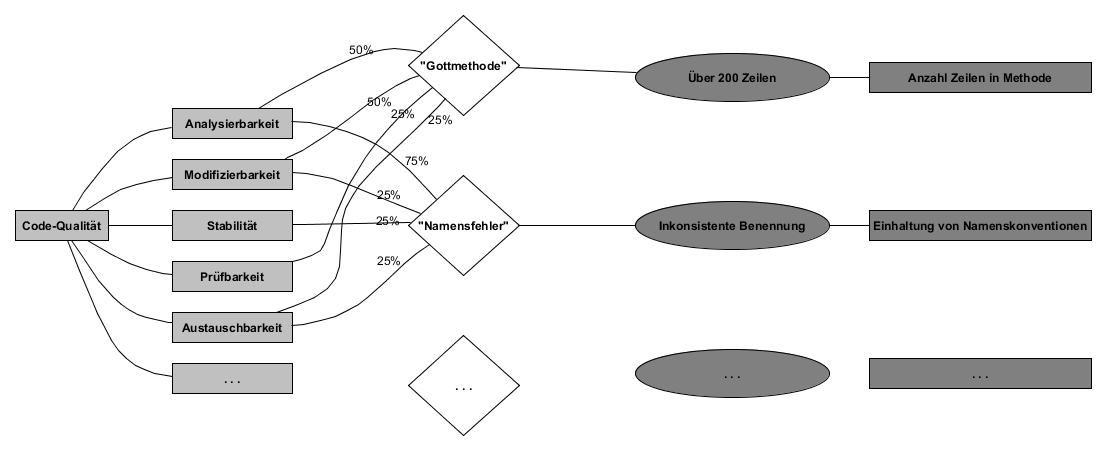
\includegraphics [width=\textwidth] {model.png}
				\caption{Ausschnitt des für den Code-Quality-Index verwendeten Qualitätsmodells mit Qualitätseigenschaften, Qualitätsindikatoren, Problemmustern und Qualitätsmerkmalen (von links nach rechts)}
				\label{qualitymodel}
			\end{figure}
			\subsection{Qualitätsindikatoren}
				Die 52 Qualitätsindikatoren aus denen sich der Index zusammensetzt enthalten also jeweils ein zugeordnetes Problemmuster als Definition, und die gewichtete Abbildung auf die Qualitätseigenschaften von null bis einhundert Prozent, wobei die Abstufung jeweils in 25 Prozent Schritten erfolgt. Darüber hinaus wurde für alle Indikatoren analysiert wie hoch der Aufwand zur Behebung des Problemmusters ist ("`Kostenzuwachs"') und wie unmittelbar sich eine Behebung positiv auswirkt. Beides wurde analog zur Skala für die Qualitätseigenschaften eingestuft. Abschließend wurden über 120 Industrieprojekte hinsichtlich der Problemmuster vermessen und die Ergebnisse in einer Datenbank abgelegt. Dabei wurden die Fehlerhäufigkeiten jeweils mittels der Anzahl der Codezeilen des vermessenen Systems normiert, um vergleichbare Werte zu erhalten und so aufbereitet, dass sich ein neu zu untersuchendes System im Vergleich zu dieser Datenbasis einordnen lässt. Dafür wurde erneut auf die Abstufung in 25 Prozent Schritten zurückgegriffen, sodass sich bezüglich jedes Indikators aussagen lässt, ob das vermessene Programm besser als 25, 50, 75 oder 100 Prozent der Programme in der Datenbasis ist. Diese Grenzen werden als "`Schwellwerte"' bezeichnet. \newline
			Als Beispiel sei hier der Qualitätsindikator "`duplizierter Code"' aufgeführt, der folgendermaßen definiert ist \cite{CodeQualityManagement}:
				\begin{quote}
  					"`Duplizierter Code liegt vor, wenn mindestens 40 aufeinander folgende Codezeilen (inkl. Leerzeilen und Kommentarzeilen) innerhalb des Quellcodes in identischer Form mehrmals auftreten."'
  				\end{quote}
  				\begin{figure} [h]
					\centering
					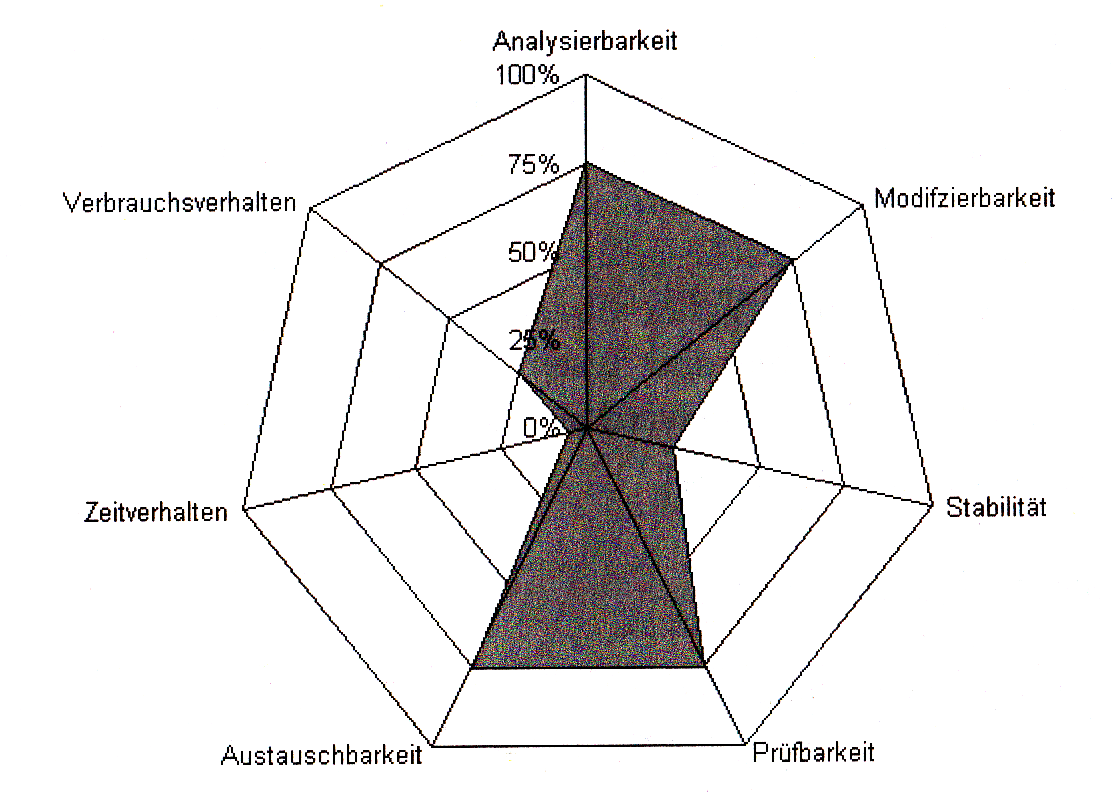
\includegraphics [width=0.6\textwidth] {indexeigenschaften.png}
					\caption{Zuordnung des Problemmusters "`duplizierter Code"' zu den Qualitätseigenschaften \cite{CodeQualityManagement}}
					\label{indexeigen}
				\end{figure}
				Die Zuordnung zu den Qualitätseigenschaften wird mittels Kiviatdiagramm dargestellt (siehe Abbildung~\ref{indexeigen}). Der Kostenzuwachs wurde mit 50 Prozent bewertet, die Unmittelbarkeit mit 75 Prozent. Abbildung~\ref{indexschwell} beinhaltet die Häufigkeit des Problemmusters in der Datenbasis (für Java-Programme). \newline
				\begin{figure} [h]
					\centering
					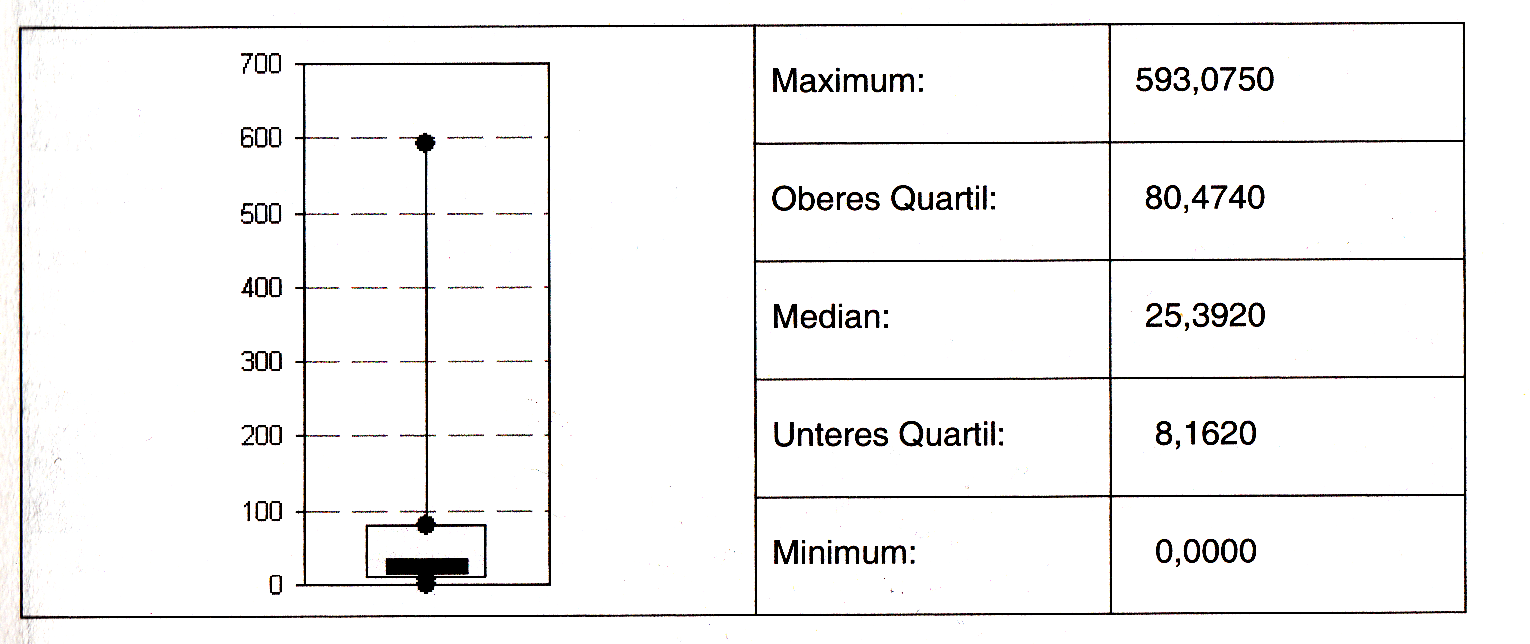
\includegraphics [width=\textwidth] {indexschwellwerte.png}
					\caption{Anzahl duplizierter Codezeilen je 1000 Zeilen Code in Datenbasis \cite{CodeQualityManagement}}
					\label{indexschwell}
				\end{figure}
			\subsection{Index-Definition}
				Um anhand der Messergebnisse für die Indikatoren eine Gesamteinstufung in Form eines einfachen Indexes zu ermöglichen, wurden fünf Quality-Benchmark-Level (QBL) definiert (siehe Tabelle~\ref{indexlevel}) deren Erreichbarkeit über zwei Mechanismen gesteuert wird:
				\begin{itemize}
					\item \textbf{Indikatorzuwachs} Mit jedem Level kommen weitere Indikatoren hinzu, abhängig davon welche Qualitätseigenschaften sie beeinflussen. Je nach Kostenzuwachs und Unmittelbarkeit können Indikatoren darüber hinaus vorgezogen oder in höhere Level verschoben werden (unmittelbar wirkende, schnell zu korrigierende Indikatoren werden bevorzugt).
					\item \textbf{Schwellwerttunnel} Je höher der zu erreichende Level, desto besser muss das vermessene Programm im Vergleich zur Datenbasis für die relevanten Indikatoren abschneiden (25\% für QBL 2 bis 100\% für QBL 5). 
				\end{itemize}
				\begin{center}
					\tabulinesep=1.5mm
					\begin{longtabu}{|c|c|c|c|}
						\hline
  						\textbf{Level} & \textbf{Bezeichnung} & \textbf{Beschreibung} & \textbf{Eigenschaften} \\
  						\hline 
						QBL 1 & Rudimentary & komplierfähiges, ausführbares Programm & - \\  						
  						\hline
  						QBL 2 & Basic & Minimum an Code-Qualität für & Analysierbarkeit \\ & & wirtschaftliche Anpassbarkeit & Stabilität \\
  						\hline
  						QBL 3 & Extended & gute technische Qualität, & Zeitverhalten \\ & & technisch Zukunftsfähig & Verbrauchsverhalten \\
  						\hline
  						QBL 4 & Advanced & hervorragende Qualität, explizite & Prüfbarkeit \\ & & Struktur für Weiterentwicklung & Modifizierbarkeit \\
  						\hline
  						QBL 5 & Complete & perfekte Qualität, Struktur für & Austauschbarkeit \\ & & Weiterentwicklung und Wiederverwendung & \\
  						\hline
  						\caption{Für den Code-Quality-Index definierte Level \cite{CodeQualityManagement}}
						\label{indexlevel}
  					\end{longtabu}   
  				\end{center}
  				\newpage
		\section{Verwendung und Bewertung in der Praxis}
			Vorab lässt sich sagen, dass der Code-Quality-Index in dieser Form weder zu einem weitreichend akzeptiertem Standard geworden ist, noch vielfältige Anwendung in der Wirtschaft gefunden hat. Auch die von den Autoren angestrebte Fortführung der angefangenen Datenbasis ist anscheinend nicht langfristig durchgeführt worden. Der im Buch genannte Webauftritt ist nicht mehr erreichbar. \newline
			Allerdings gab es mindestens eine Umsetzung für ein produktives System. Für die IT-Infrastruktur der Dresdener Bank, also die Bereitstellung von Online-Funktionen und Informationen für Endkunden und Mitarbeiter innerhalb einer J2EE-Architektur wurde Code-Quality-Management in Form des beschriebenen Indexes durch die SQS AG etabliert und damit zufriedenstellende Ergebnisse erreicht \cite{DresdnerBank}. Allerdings wurde hierbei festgestellt, dass die Auswahl und konkrete Ausprägung der Indikatoren für den Kontext angepasst werden müssen. Die 52 Indikatoren von Frank Simon et Al. können nicht als allgemeingültig betrachtet werden. \newline
			Eine weniger praxisnahe, aber vollständige Umsetzung des Code-Quality-Index erfolgte im Rahmen der Diplomarbeit von Torsten Möllenbeck an der Universität Bremen \cite{DAIndexUmsetzung}. Diese zeigt, dass es auf jeden Fall möglich ist, den Index vollständig automatisiert zu ermitteln, auch wenn leider nur Ergebnisse von C++ Programmen ausgewertet wurden. Allerdings werden einige Kritikpunkte an der Konzeption des Indexes angebracht, die ihre Berechtigung haben:
			\begin{itemize}
				\item Die dynamischen Schwellwerte abhängig von der Datenbasis können dazu führen, dass Systeme nachträglich anders eingestuft würden, wenn weitere besonders gute oder besonders schlechte Programme hinzugefügt werden. Mit Blick auf das Softwarepraktikum bedeutet dies, dass die Datenbasis zumindest über den Verlauf eines Softwarepraktikums konstant gehalten werden muss um eine gerechte und stabile Bewertung vorzunehmen und darüber hinaus die Entwicklung der Qualität im Verlauf des Praktikums zu untersuchen.
				\item Der Aufbau des Indexes kann dazu führen, dass ein System das bezüglich fast aller Indikatoren eine hervorragende Qualität aufweist aber in einem einzigen Indikator sehr schlecht ist, beziehungsweise bewusst von einer Regel abweicht auf dem untersten Level eingestuft wird. Es erscheint daher sinnvoll, den Index kontextspezifisch anzupassen wenn die Notwendigkeit besteht.
				\item Auch wenn die Problemmuster durch die Autoren gut belegt sind, erscheinen einige der gewählten Grenzwerte recht willkürlich und damit auch fragwürdig. Als Beispiel sei hier der Indikator "`falsche Namenslänge"' genannt, bei dem es sicher verschiedene Meinungen zu der Frage gibt ob 50 Zeichen wirklich eine sinnvolle Grenze sind. Auch hier bietet sich eine spezifische Anpassung für das zu bewertende System an.
			\end{itemize}
			Trotz dieser Schwächen und dem nicht erfüllten Universalitätsanspruch finden sich einige Umsetzungen ähnlicher Bewertungssysteme. So wurde durch Ana Dragomir und Horst Lichter an der Universität Aachen ein Index für die Beurteilung von Softwarearchitekturen vorgeschlagen \cite{ArchitectureIndex}. \newline
			Ein sehr ähnliches Vorgehen wie beim Code-Quality-Index verfolgen Baggen et Al. mit ihrem Code-Benchmark \cite{CodeBenchmark}. Es werden ebenso Indikatoren gebildet und auf beeinflusste Qualitätseigenschaften abgebildet, allerdings werden hier sehr viel weniger und allgemeinere Indikatoren verwendet. Ein etwas neuerer Ansatz aus der Wirtschaft stammt von der Firma TIOBE die mit ihrem TIOBE Quality Indicator ebenfalls weniger Indikatoren definieren als im Code-Quality-Index \cite{TIOBEIndex}. Allerdings werden für die erreichbaren Stufen keine Indikatoren ausgewählt sondern es werden immer alle vermessen. Unterschiedlich ist dabei dann lediglich der zu erreichende Schwellwert. Für die Gesamtbewertung wurde darüber hinaus noch eine Wichtung der Indikatoren vorgenommen. Als hervorstechendes Merkmal sei hier die ansprechende Präsentation des Ergebnisses genannt, dass an die Energieeffizienz-Plaketten von elektrischen Geräten erinnert (Siehe Abbildung~\ref{TIOBElabel}). \newline
			\begin{figure} [h]
				\centering
				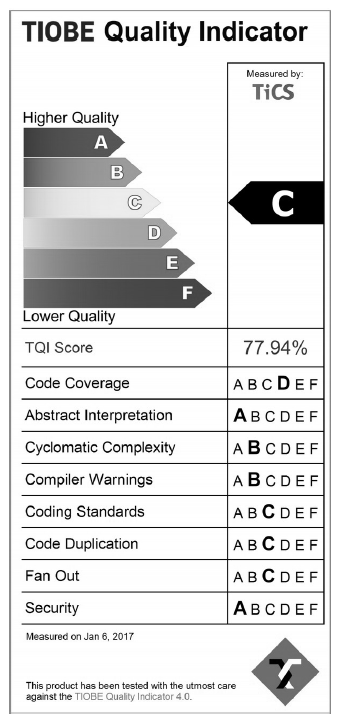
\includegraphics [width=0.4\textwidth] {tiobe.png}
				\caption{TIOBE Quality Indicator Ergebnisdarstellung \cite{TIOBEIndex}}
				\label{TIOBElabel}
			\end{figure}
		\section{Anpassung für das Softwarepraktikum}
			Die Anwendung des Code-Quality-Index in anderen Projekten und vergleichbare Ansätze machen ebenso deutlich wie die vom Indikatorkatalog abweichende Regelwerkdefinition, dass für das Softwarepraktikum der Code-Quality-Index nicht einfach übernommen werden kann, sondern entsprechend den speziellen Anforderungen und Möglichkeiten in diesem Rahmen angepasst werden muss. \newline
			Zunächst fällt auf, dass sich die gewählten Regeln nicht ohne weiteres auf das bidirektionale Qualitätsmodell von Simon et Al. abbilden lassen. Es müsste für die im Original nicht verwendeten Regeln aufwendig neu erforscht werden. Außerdem ist dieses Modell für die einführende Lehrveranstaltung zu komplex um es den Studenten erschöpfend zu vermitteln. Die Zuordnung der Regeln beziehungsweise Indikatoren als Mengen von Regeln zu einem Benchmark-Level muss daher über einen anderen Mechanismus erfolgen. Die einfachste und naheliegende Möglichkeit dafür bilden die Einstufungen der Regeln nach Schweregrad, sodass "`Blocker"'-Regeln bereits für den Level zwei und "`Info"'-Regeln erst für den Level vier relevant sind. Die Verschiebung der Regeln je nach Unmittelbarkeit und Kostenzuwachs entfällt in diesem Kontext vollständig, da dies ebenso neu ermittelt werden müsste und im Kontext des Softwarepraktikums mit dem gewählten Regelwerk ohnehin keine große Rolle spielt. \newline
			Eine weitere Anpassung betrifft die Schwellwerte. Da es in der Lehre nicht üblich ist, für die beste Note 100 Prozent zu verlangen, erscheint dies auch für den Code-Quality-Index als zu strenge Forderung. Daher wurde zusätzlich der Schwellwert "`Besser als 90\%"' eingeführt um eine adäquate Bewertung vorzunehmen. Tabelle~\ref{indexdef} enthält die mit dem Lehrstuhl abgestimmte Neudefinition der Benchmark-Level für das Softwarepraktikum. Da sich bei der Vermessung der Praktikumsprojekte der letzten 2 Jahrgänge herausstellte, dass diese Schwellwerte dazu führen, dass bis auf eine Gruppe alle nur Level eins erreichen und die Index-Einstufung so keine Aussagekraft haben kann wurden die Schwellwerte stattdessen in 10-Prozent-Schritten ermittelt und die Zuordnung zu den Benchmark-Level über die angelegte Datenbank konfigurierbar gemacht. Mit der in Tabelle~\ref{indexdefnew} festgelegten Zuordnung erreichen die Gruppen Einstufungen zwischen Level eins und Level vier. \newline 
			\begin{center}
				\tabulinesep=1.5mm
				\begin{longtabu}{|c|c|c|c|}
					\hline
  					\textbf{Level} & \textbf{Bezeichnung} & \textbf{Beschreibung} \\
  					\hline 
					QBL 1 & Mangelhaft & komplierfähiges, ausführbares Programm \\  						\hline
  					QBL 2 & Ausreichend & 50\% Blocker, 25\% Critical \\ 
  					\hline
  					QBL 3 & Befriedigend & 75\% Blocker, 50\% Critical, 50\% Major, 25\% Minor \\
  					\hline
  					QBL 4 & Gut & 90\% Blocker, 75\% Critical, 75\% Major, 50\% Minor, 50\% Info \\
  					\hline
  					QBL 5 & Sehr Gut & 100\% Blocker, 100\% Critical, 90\% Major, 90\% Minor, 90\% Info \\
  					\hline
  					\caption{Neudefinition der Benchmark-Level für das Softwarepraktikum vor der Vermessung}
					\label{indexdef}
  				\end{longtabu}   
  			\end{center}
  			\begin{center}
				\tabulinesep=1.5mm
				\begin{longtabu}{|c|c|c|c|}
					\hline
  					\textbf{Level} & \textbf{Bezeichnung} & \textbf{Beschreibung} \\
  					\hline 
					QBL 1 & Mangelhaft & komplierfähiges, ausführbares Programm \\  						\hline
  					QBL 2 & Ausreichend & 10\% Blocker \\ 
  					\hline
  					QBL 3 & Befriedigend & 20\% Blocker, 10\% Critical, 10\% Major \\
  					\hline
  					QBL 4 & Gut & 30\% Blocker, 30\% Critical, 20\% Major, 10\% Minor \\
  					\hline
  					QBL 5 & Sehr Gut & 50\% Blocker, 40\% Critical, 30\% Major, 20\% Minor, 10\% Info \\
  					\hline
  					\caption{Für die Vermessung verwendete Definition der Benchmark-Level, die eine annehmbare Verteilung der Bewertungen erzeugt}
					\label{indexdefnew}
  				\end{longtabu}   
  			\end{center}
  			Dieses starke Herabsetzen der Grenzen zum Erreichen eines höheren Benchmark-Level ist notwendig, da in den vermessenen Projekten keine Gruppe dabei war, die bezüglich aller Indikatoren im oberen Bereich liegt. Die meisten Gruppen sind bezüglich einiger weniger Indikatoren sehr gut, dafür aber bezüglich der meisten anderen nur Mittelfeld. Interessanterweise sind die gut erfüllten Indikatoren nicht immer die Gleichen, sondern sehr unterschiedlich. Dadurch entstehen im Aufbau der Datenbank anspruchsvolle Zielwerte für alle Indikatoren, die dann von keiner Gruppe bezüglich aller Indikatoren eingehalten werden. Wenn das neue Regelwerk in Zukunft kommuniziert und von den Studenten angewendet wird, ist es möglich, dass eine nachträgliche Anpassung der Zuordnungen sinnvoll wird. \newline
  			Im Folgenden werden die definierten Indikatoren kurz vorgestellt. Die genannten SonarQube-Regeln finden sich in der Dokumentation des Java-Plugins \cite{JavaPlugin}. Die angegebenen Tabellen sind dabei so zu lesen, dass ein Programm besser als die in der oberen Zeile angegeben Prozent der Programme in der Datenbasis ist, wenn die Häufigkeit des Problemmusters je 1000 Netto-Code-Zeilen geringer als der in der unteren Zeile angegebene Wert ist. Der Wert für null Prozent ist also das in Bezug auf diesen Indikator schlechteste vermessene Programm, und der Wert für einhundert Prozent das Beste in der Datenbasis. Für Indikatoren bei denen mehrere Schwellwerte identisch sind wurden die entsprechenden Tabelleneinträge zusammengefasst.\newline
  			\subsection{Indikator Magic Numbers}
  				Klasse: "`Blocker"' \newline
  				Entspricht der SonarQube-Regel "`Magic numbers should not be used"' und hat im Original-Index keine Entsprechung. Aufgrund der im Softwarepraktikum verwendeten Daten-Initialisierung durch eine Klasse mit dem Prefix "`DataInitializer"' in der sehr viele Zahlen im Code stehen ohne das dies ein Problem darstellt werden die Regelverletzungen in diesen Klassen für den Index ignoriert.
  				\begin{center}
					\tabulinesep=1.5mm
					\begin{longtabu}{c|c|c|c|c|c|c}
						\hline
  						\multicolumn1{|l|}{\textbf{Besser als}} & 0\% & 10\% & 20\% & 30\% & 40\% & \multicolumn1{c|}{50\%} \\
  						\hline
  						\multicolumn1{|l|}{\textbf{Häufigkeit}} & 79,771 & 25,179 & 16,248 & 13,127 & 11,275 & \multicolumn1{c|}{8,922} \\
  						\hline
  						\multicolumn{7}{c}{} \\
  						\hline
  						\multicolumn1{|l|}{\textbf{Besser als}} & 60\% & 70\% & 80\% & 90\% & 100\% & \multicolumn1{c|}{}\\
  						\hline
  						\multicolumn1{|l|}{\textbf{Häufigkeit}} & 6,890 & 3,968 & 2,677 & 1,054 & 0,000 & \multicolumn1{c|}{}\\
  						\hline
  						\caption{Ermittelter Schwellwerttunnel für Indikator Magic Numbers}
  					\end{longtabu}   
  				\end{center}
  				\newpage
  			\subsection{Indikator Duplizierter Code}
  				Klasse: "`Blocker"' \newline
  				Entspricht der SonarQube-Regel "`Source files should not have any duplicated blocks"' wobei im Gegensatz zum Original-Index die Anzahl der duplizierten Code-Blöcke gezählt wird und nicht die Anzahl der darin enthaltenen Zeilen. 
  				\begin{center}
					\tabulinesep=1.5mm
					\begin{longtabu}{c|c|c|c|c|c|c}
						\hline
  						\multicolumn1{|l|}{\textbf{Besser als}} & 0\% & 10\% & 20\% & 30\% & 40\% & \multicolumn1{c|}{50\%} \\
  						\hline
  						\multicolumn1{|l|}{\textbf{Häufigkeit}} & 3,454 & 2,965 & 2,230 & 1,891 & 1,605 & \multicolumn1{c|}{1,446} \\
  						\hline
  						\multicolumn{7}{c}{} \\
  						\hline
  						\multicolumn1{|l|}{\textbf{Besser als}} & 60\% & 70\% & 80\% & 90\% & 100\% & \multicolumn1{c|}{}\\
  						\hline
  						\multicolumn1{|l|}{\textbf{Häufigkeit}} & 1,181 & 0,935 & 0,717 & 0,259 & 0,000 & \multicolumn1{c|}{}\\
  						\hline
  						\caption{Ermittelter Schwellwerttunnel für Indikator Duplizierter Code}
  					\end{longtabu}   
  				\end{center}
  			\subsection{Indikator Datenkapselaufbruch}
  				Klasse: "`Blocker"' \newline
  				Entspricht der SonarQube-Regel "`Class variable fields should not have public accessibility"' und ist in seiner Bedeutung identisch zum Original.
  				\begin{center}
					\tabulinesep=1.5mm
					\begin{longtabu}{c|c|c|c|c|c|c}
						\hline
  						\multicolumn1{|l|}{\textbf{Besser als}} & 0\% & 10\% & 20\% & 30\% & 40\% & \multicolumn1{c|}{50\% - 100\%} \\
  						\hline
  						\multicolumn1{|l|}{\textbf{Häufigkeit}} & 6,430 & 1,613 & 0,836 & 0,590 & 0,178 & \multicolumn1{c|}{0,000} \\
  						\hline
  						\caption{Ermittelter Schwellwerttunnel für Indikator Datenkapselaufbruch}
  					\end{longtabu}   
  				\end{center}
  			\subsection{Indikator Überbuchte Datei}
  				Klasse: "`Critical"' \newline
  				Entspricht der SonarQube-Regel "`Files should contain only one top-level class or interface each"' und ist in seiner Bedeutung identisch zum Original.
  				\begin{center}
					\tabulinesep=1.5mm
					\begin{longtabu}{c|c}
						\hline
  						\multicolumn1{|l|}{\textbf{Besser als}} &  \multicolumn1{c|}{0\% - 100\%} \\
  						\hline
  						\multicolumn1{|l|}{\textbf{Häufigkeit}} & \multicolumn1{c|}{0,000} \\
  						\hline
  						\caption{Ermittelter Schwellwerttunnel für Indikator Überbuchte Datei}
  					\end{longtabu}   
  				\end{center}
  			\subsection{Indikator Unzureichende Tests}
  				Klasse: "`Critical"' \newline
  				Entspricht der SonarQube-Regel "`Lines should have sufficient coverage by unit tests"' und hat im Original-Index keine Entsprechung. Als ausreichende Testabdeckung wird im Kontext des Softwarepraktikums 80\% festgelegt. Dieser Grenzwert bewegt sich im Mittelfeld der in der Literatur genannten Werte und wurde vom Lehrstuhl so festgelegt. 
  				\begin{center}
					\tabulinesep=1.5mm
					\begin{longtabu}{c|c|c|c|c|c|c}
						\hline
  						\multicolumn1{|l|}{\textbf{Besser als}} & 0\% & 10\% & 20\% & 30\% & 40\% & \multicolumn1{c|}{50\%} \\
  						\hline
  						\multicolumn1{|l|}{\textbf{Häufigkeit}} & 14,970 & 13,109 & 10,375 & 9,708 & 8,322 & \multicolumn1{c|}{7,976} \\
  						\hline
  						\multicolumn{7}{c}{} \\
  						\hline
  						\multicolumn1{|l|}{\textbf{Besser als}} & 60\% & 70\% & 80\% & 90\% & 100\% & \multicolumn1{c|}{}\\
  						\hline
  						\multicolumn1{|l|}{\textbf{Häufigkeit}} & 6,815 & 6,217 & 4,748 & 2,893 & 0,000 & \multicolumn1{c|}{}\\
  						\hline
  						\caption{Ermittelter Schwellwerttunnel für Indikator Unzureichende Tests}
  					\end{longtabu}   
  				\end{center}
  			\subsection{Indikator Zu enge Kopplung}
  				Klasse: "`Critical"' \newline
  				Enthält die beiden SonarQube-Regeln "`Classes should not be coupled to too many other classes (Single Responsibility Principle)"' und "`Cycles between packages should be removed"', wobei letztere dem Indikator "`Verbotene Paketliebe"' entspricht. Die enge thematische Zusammengehörigkeit führte zur Zusammenlegung.
  				\begin{center}
					\tabulinesep=1.5mm
					\begin{longtabu}{c|c|c|c|c|c|c}
						\hline
  						\multicolumn1{|l|}{\textbf{Besser als}} & 0\% & 10\% & 20\% & 30\% & 40\% & \multicolumn1{c|}{50\%} \\
  						\hline
  						\multicolumn1{|l|}{\textbf{Häufigkeit}} & 16,750 & 10,256 & 8,740 & 7,133 & 6,810 & \multicolumn1{c|}{6,554} \\
  						\hline
  						\multicolumn{7}{c}{} \\
  						\hline
  						\multicolumn1{|l|}{\textbf{Besser als}} & 60\% & 70\% & 80\% & 90\% & 100\% & \multicolumn1{c|}{}\\
  						\hline
  						\multicolumn1{|l|}{\textbf{Häufigkeit}} & 6,117 & 5,606 & 4,835 & 3,978 & 3,310 & \multicolumn1{c|}{}\\
  						\hline
  						\caption{Ermittelter Schwellwerttunnel für Indikator Zu enge Kopplung}
  					\end{longtabu}   
  				\end{center}
  				\newpage
  			\subsection{Indikator Gottkonstrukt}
  				Klasse: "`Critical"' \newline
  				Enthält vier SonarQube-Regeln, die die Größe von Dateien, Klassen, Methoden und Inneren Klassen betreffen. Bis auf die Größe von inneren Klassen finden sich für alle Regeln entsprechende Qualitätsindikatoren. Da das übergeordnete Prinzip Code-Elemente klein und übersichtlich zu halten adressiert werden soll wurden diese zusammengelegt. Die Grenzwerte orientieren sich am Softwarepraktikum in Dortmund \cite{CleanCodeImPraktikum}.
  				\begin{center}
					\tabulinesep=1.5mm
					\begin{longtabu}{c|c|c|c|c|c|c}
						\hline
  						\multicolumn1{|l|}{\textbf{Besser als}} & 0\% & 10\% & 20\% & 30\% & 40\% & \multicolumn1{c|}{50\%} \\
  						\hline
  						\multicolumn1{|l|}{\textbf{Häufigkeit}} & 9,422 & 8,936 & 8,326 & 7,565 & 7,253 & \multicolumn1{c|}{6,815} \\
  						\hline
  						\multicolumn{7}{c}{} \\
  						\hline
  						\multicolumn1{|l|}{\textbf{Besser als}} & 60\% & 70\% & 80\% & 90\% & 100\% & \multicolumn1{c|}{}\\
  						\hline
  						\multicolumn1{|l|}{\textbf{Häufigkeit}} & 6,591 & 6,065 & 5,615 & 4,937 & 3,960 & \multicolumn1{c|}{}\\
  						\hline
  						\caption{Ermittelter Schwellwerttunnel für Indikator Gottkonstrukt}
  					\end{longtabu}   
  				\end{center}
  				\subsection{Indikator Namensfehler} 
  				Klasse: "`Critical"' \newline
  				Enthält alle SonarQube-Regeln bezüglich Namenskonventionen und entspricht im wesentlichen dem Original. Die Standard-Java-Pattern wurden um die Größenbeschränkung gemäß dem Original-Indikator "`Falsche Namenslänge"' erweitert. Eine separate Messung dieses Indikators ist mit den vordefinierten Java-Regeln in SonarQube nicht möglich. 
  				\begin{center}
					\tabulinesep=1.5mm
					\begin{longtabu}{c|c|c|c|c|c|c}
						\hline
  						\multicolumn1{|l|}{\textbf{Besser als}} & 0\% & 10\% & 20\% & 30\% & 40\% & \multicolumn1{c|}{50\%} \\
  						\hline
  						\multicolumn1{|l|}{\textbf{Häufigkeit}} & 57,931 & 38,099 & 27,724 & 21,749 & 14,811 & \multicolumn1{c|}{13,559} \\
  						\hline
  						\multicolumn{7}{c}{} \\
  						\hline
  						\multicolumn1{|l|}{\textbf{Besser als}} & 60\% & 70\% & 80\% & 90\% & 100\% & \multicolumn1{c|}{}\\
  						\hline
  						\multicolumn1{|l|}{\textbf{Häufigkeit}} & 11,245 & 9,592 & 6,969 & 5,347 & 1,123 & \multicolumn1{c|}{}\\
  						\hline
  						\caption{Ermittelter Schwellwerttunnel für Indikator Namensfehler}
  					\end{longtabu}   
  				\end{center}
  				\newpage
  			\subsection{Indikator Informelle Dokumentation}
  				Klasse: "`Critical"' \newline
  				Entspricht der SonarQube-Regel "`Public types, methods and fields (API) should be documented with Javadoc"' und ist in seiner Bedeutung identisch zum Original.
  				\begin{center}
					\tabulinesep=1.5mm
					\begin{longtabu}{c|c|c|c|c|c|c}
						\hline
  						\multicolumn1{|l|}{\textbf{Besser als}} & 0\% & 10\% & 20\% & 30\% & 40\% & \multicolumn1{c|}{50\%} \\
  						\hline
  						\multicolumn1{|l|}{\textbf{Häufigkeit}} & 63,249 & 51,517 & 44,137 & 32,258 & 25,868 & \multicolumn1{c|}{23,948} \\
  						\hline
  						\multicolumn{7}{c}{} \\
  						\hline
  						\multicolumn1{|l|}{\textbf{Besser als}} & 60\% & 70\% & 80\% & 90\% & 100\% & \multicolumn1{c|}{}\\
  						\hline
  						\multicolumn1{|l|}{\textbf{Häufigkeit}} & 21,304 & 12,335 & 8,854 & 3,954  & 0,000 & \multicolumn1{c|}{}\\
  						\hline
  						\caption{Ermittelter Schwellwerttunnel für Indikator Informelle Dokumentation}
  					\end{longtabu}   
  				\end{center}
  			\subsection{Indikator Verwechslungsgefahr}
  				Klasse: "`Major"' \newline
  				Enthält alle SonarQube-Regeln, die die Überdeckung von Bezeichnern in untergeordneten Geltungsbereichen verbieten, sowie die Forderung, dass sich Bezeichner nicht nur in Groß- und Kleinschreibung unterscheiden dürfen und dass ein Datentyp-Suffix wie "`L"' für Long groß geschrieben werden soll. All diese Regeln haben zum Ziel Verwechslungen zu vermeiden. 
  				\begin{center}
					\tabulinesep=1.5mm
					\begin{longtabu}{c|c|c|c|c|c|c|c|c}
						\hline
  						\multicolumn1{|l|}{\textbf{Besser als}} & 0\% & 10\% & 20\% & 30\% & 40\% & 50\% & 60\% & \multicolumn1{c|}{70\% - 100\%} \\
  						\hline
  						\multicolumn1{|l|}{\textbf{Häufigkeit}} & 17,839 & 2,687 & 1,497 & 0,554 & 0,494 & 0,356 & 0,278 & \multicolumn1{c|}{0,000} \\
  						\hline
  						\caption{Ermittelter Schwellwerttunnel für Indikator Verwechslungsgefahr}
  					\end{longtabu}   
  				\end{center}
  			\subsection{Indikator Formatierungsfehler}
  				Klasse: "`Major"' \newline
  				Enthält SonarQube-Regeln bezüglich der Setzung von geschweiften Klammern, Einrückung und Zeilenlänge. Keine der ausgewählten Regeln hat eine Entsprechung im Original Index.
  				\begin{center}
					\tabulinesep=1.5mm
					\begin{longtabu}{c|c|c|c|c|c|c}
						\hline
  						\multicolumn1{|l|}{\textbf{Besser als}} & 0\% & 10\% & 20\% & 30\% & 40\% & \multicolumn1{c|}{50\%} \\
  						\hline
  						\multicolumn1{|l|}{\textbf{Häufigkeit}} & 288,193 & 243,131 & 232,493 & 222,187 & 209,668 & \multicolumn1{c|}{200,345} \\
  						\hline
  						\multicolumn{7}{c}{} \\
  						\hline
  						\multicolumn1{|l|}{\textbf{Besser als}} & 60\% & 70\% & 80\% & 90\% & 100\% & \multicolumn1{c|}{}\\
  						\hline
  						\multicolumn1{|l|}{\textbf{Häufigkeit}} & 183,627 & 173,311 & 149,972 & 51,639 & 0,000 & \multicolumn1{c|}{}\\
  						\hline
  						\caption{Ermittelter Schwellwerttunnel für Indikator Formatierungsfehler}
  					\end{longtabu}   
  				\end{center}
  			\subsection{Indikator Zu Komplex}
  				Klasse: "`Major"' \newline
  				Enthält SonarQube-Regeln zur Verschachtelungstiefe von Kontrollflussanweisungen, Parameteranzahl von Methoden sowie die McCabe-Komplexität für Methoden und Klassen. Die Original-Indikatoren "`Labyrinthmethode"' und "`Lange Parameterliste"' sind Teil dieses Indikators.
  				\begin{center}
					\tabulinesep=1.5mm
					\begin{longtabu}{c|c|c|c|c|c|c}
						\hline
  						\multicolumn1{|l|}{\textbf{Besser als}} & 0\% & 10\% & 20\% & 30\% & 40\% & \multicolumn1{c|}{50\%} \\
  						\hline
  						\multicolumn1{|l|}{\textbf{Häufigkeit}} & 20,474 & 11,787 & 9,251 & 8,276 & 7,376 & \multicolumn1{c|}{6,890} \\
  						\hline
  						\multicolumn{7}{c}{} \\
  						\hline
  						\multicolumn1{|l|}{\textbf{Besser als}} & 60\% & 70\% & 80\% & 90\% & 100\% & \multicolumn1{c|}{}\\
  						\hline
  						\multicolumn1{|l|}{\textbf{Häufigkeit}} & 6,054 & 5,039 & 3,881 & 3,208 & 2,109 & \multicolumn1{c|}{}\\
  						\hline
  						\caption{Ermittelter Schwellwerttunnel für Indikator Zu Komplex}
  					\end{longtabu}   
  				\end{center}
  			\subsection{Indikator Objektplacebo}
  				Klasse: "`Minor"' \newline
  				Entspricht der SonarQube-Regel "`"static" members should be accessed statically"' und ist in seiner Bedeutung identisch zum Original.
  				\begin{center}
					\tabulinesep=1.5mm
					\begin{longtabu}{c|c|c|c}
						\hline
  						\multicolumn1{|l|}{\textbf{Besser als}} & 0\% & 10\% & \multicolumn1{c|}{20\% - 100\%} \\
  						\hline
  						\multicolumn1{|l|}{\textbf{Häufigkeit}} & 6,366 & 0,277 & \multicolumn1{c|}{0,000} \\
  						\hline
  						\caption{Ermittelter Schwellwerttunnel für Indikator Objektplacebo}
  					\end{longtabu}   
  				\end{center}
  			\subsection{Indikator Objektvergleich}
  				Klasse: "`Minor"' \newline
  				Entspricht der SonarQube-Regel "`Objects should be compared with equals()"' und hat im Original-Index keine Entsprechung.
  				\begin{center}
					\tabulinesep=1.5mm
					\begin{longtabu}{c|c|c|c|c|c|c|c}
						\hline
  						\multicolumn1{|l|}{\textbf{Besser als}} & 0\% & 10\% & 20\% & 30\% & 40\% & 50\% & \multicolumn1{c|}{60\% - 100\%} \\
  						\hline
  						\multicolumn1{|l|}{\textbf{Häufigkeit}} & 4,970 & 2,673 & 1,248 & 0,777 & 0,503 & 0,216 & \multicolumn1{c|}{0,000} \\
  						\hline
  						\caption{Ermittelter Schwellwerttunnel für Indikator Objektvergleich}
  					\end{longtabu}   
  				\end{center}
  			\subsection{Indikator Risikocode}
  				Klasse: "`Minor"' \newline
  				Enthält die beiden SonarQube-Regeln "`switch statements should end with default clauses"' und "`Switch cases should end with an unconditional break statement"'. Damit werden zwei drittel des Original-Indikators abgedeckt.
  				\begin{center}
					\tabulinesep=1.5mm
					\begin{longtabu}{c|c|c|c|c|c}
						\hline
  						\multicolumn1{|l|}{\textbf{Besser als}} & 0\% & 10\% & 20\% & 30\% & \multicolumn1{c|}{40\% - 100\%} \\
  						\hline
  						\multicolumn1{|l|}{\textbf{Häufigkeit}} & 6,609 & 0,948 & 0,433 & 0,182 & \multicolumn1{c|}{0,000} \\
  						\hline
  						\caption{Ermittelter Schwellwerttunnel für Indikator Risikocode}
  					\end{longtabu}   
  				\end{center}
  			\subsection{Indikator Importfehler}
  				Klasse: "`Minor"' \newline
  				Enthält die beiden SonarQube-Regeln "`Useless imports should be removed"' und "`Wildcard imports should not be used"'. Damit stellt dieser Indikator eine Mischung, aber nicht vollständige Abdeckung der Original-Indikatoren "`Importlüge"' und "`Importchaos"' dar.
  				\begin{center}
					\tabulinesep=1.5mm
					\begin{longtabu}{c|c|c|c|c|c|c|c|c|c}
						\hline
  						\multicolumn1{|l|}{\textbf{Besser als}} & 0\% & 10\% & 20\% & 30\% & 40\% & 50\% & 60\% & 70\% &\multicolumn1{c|}{80\% - 100\%} \\
  						\hline
  						\multicolumn1{|l|}{\textbf{Häufigkeit}} & 40,994 & 20,185 & 13,312 & 9,169 & 4,853 & 3,559 & 1,593 & 0,665 & \multicolumn1{c|}{0,000} \\
  						\hline
  						\caption{Ermittelter Schwellwerttunnel für Indikator Importfehler}
  					\end{longtabu}   
  				\end{center}
			\subsection{Indikator Deklarationsfehler}
				Klasse: "`Minor"' \newline
				Enthält die Forderungen nach expliziter Deklaration der Sichtbarkeit, Deklaration so spät wie möglich und nur einer Variablendeklaration pro Anweisung. Es gibt keine Entsprechung im Original-Index.
				\begin{center}
					\tabulinesep=1.5mm
					\begin{longtabu}{c|c|c|c|c|c}
						\hline
  						\multicolumn1{|l|}{\textbf{Besser als}} & 0\% & 10\% & 20\% & 30\% & \multicolumn1{c|}{40\%} \\
  						\hline
  						\multicolumn1{|l|}{\textbf{Häufigkeit}} & 15,164 & 8,603 & 4,812 & 3,924 & \multicolumn1{c|}{3,029} \\
  						\hline
  						\multicolumn{6}{c}{} \\
  						\hline
  						\multicolumn1{|l|}{\textbf{Besser als}} & 50\% & 60\% & 70\% & 80\% & \multicolumn1{c|}{90\% - 100\%}\\
  						\hline
  						\multicolumn1{|l|}{\textbf{Häufigkeit}} & 2,494 & 1,783 & 1,386 & 1,038 & \multicolumn1{c|}{0,000}\\
  						\hline
  						\caption{Ermittelter Schwellwerttunnel für Indikator Deklarationsfehler}
  					\end{longtabu}   
  				\end{center}
			\subsection{Indikator Toter Code}
				Klasse: "`Minor"' \newline
				Enthält alle SonarQube-Regeln die das entfernen von ungenutzten Code-Elementen fordern und schließt damit die Original-Indikatoren "`Tote Attribute"', "`Tote Implementierung"' und "`Tote Methoden"' mit ein.
				\begin{center}
					\tabulinesep=1.5mm
					\begin{longtabu}{c|c|c|c|c|c|c}
						\hline
  						\multicolumn1{|l|}{\textbf{Besser als}} & 0\% & 10\% & 20\% & 30\% & 40\% & \multicolumn1{c|}{50\%} \\
  						\hline
  						\multicolumn1{|l|}{\textbf{Häufigkeit}} & 36,247 & 8,897 & 7,560 & 5,810 & 3,978 & \multicolumn1{c|}{3,427} \\
  						\hline
  						\multicolumn{7}{c}{} \\
  						\hline
  						\multicolumn1{|l|}{\textbf{Besser als}} & 60\% & 70\% & 80\% & 90\% & 100\% & \multicolumn1{c|}{}\\
  						\hline
  						\multicolumn1{|l|}{\textbf{Häufigkeit}} & 2,941 & 2,495 & 1,262 & 0,499 & 0,178 & \multicolumn1{c|}{}\\
  						\hline
  						\caption{Ermittelter Schwellwerttunnel für Indikator Toter Code}
  					\end{longtabu}   
  				\end{center}
			\subsection{Indikator Unfertiger Code}
				Klasse: "`Info"' \newline
				Enthält neben der Forderung des Original-Indikators "`TODO"'-Tags zu entfernen zusätzlich die SonarQube-Regel "`Sections of code should not be commented out"'.
				\begin{center}
					\tabulinesep=1.5mm
					\begin{longtabu}{c|c|c|c|c|c|c}
						\hline
  						\multicolumn1{|l|}{\textbf{Besser als}} & 0\% & 10\% & 20\% & 30\% & 40\% & \multicolumn1{c|}{50\%} \\
  						\hline
  						\multicolumn1{|l|}{\textbf{Häufigkeit}} & 62,675 & 18,413 & 10,456 & 6,581 & 5,992 & \multicolumn1{c|}{4,701} \\
  						\hline
  						\multicolumn{7}{c}{} \\
  						\hline
  						\multicolumn1{|l|}{\textbf{Besser als}} & 60\% & 70\% & 80\% & 90\% & 100\% & \multicolumn1{c|}{}\\
  						\hline
  						\multicolumn1{|l|}{\textbf{Häufigkeit}} & 2,900 & 1,841 & 1,386 & 0,527 & 0,000 & \multicolumn1{c|}{}\\
  						\hline
  						\caption{Ermittelter Schwellwerttunnel für Indikator Unfertiger Code}
  					\end{longtabu}   
  				\end{center}			
	\chapter{Erweiterung des SonarQube-PlugIns}
		Nach der erfolgten Festlegung auf ein Regelwerk und der Anpassung und Neudefinition des Code-Quality-Index, erfolgte die Umsetzung dieser Bestandteile im SonarQube-PlugIn, sowie die Überarbeitung und Anpassung der bestehenden Funktionen. Ziel war es ein stabil lauffähiges Programm zu erhalten, dass für den produktiven Einsatz im Softwarepraktikum geeignet ist und darüber hinaus einige Funktionen zu implementieren, um die Analyse der Metriken zu ermöglichen, beziehungsweise zu  vereinfachen. 
		\section{Integration des Regelwerks}
			Auch in der Umsetzung bildet das Regelwerk den ersten fundamentalen Schritt, der mit der PlugIn-Entwicklung noch gar nichts zu tun hat. Die ausgewählten Regeln können über die Web-Oberfläche von SonarQube einfach ausgewählt und angepasst werden. Die Entscheidende Anpassung liegt hierbei in der Auswahl der Wichtung gemäß der in Kapitel~\ref{regelauswahlchapter} vorgenommenen Klassifizierung. Darüber hinaus lassen sich für einige der Ausgewählten Regeln Grenzwerte und Pattern modifizieren. Die Ausgewählten Regeln werden in einem "`Quality-Profile"' zusammengefasst und können so für die zu vermessenden Projekte mit einem Klick ausgewählt werden. So ist es auch ohne weiteres möglich Das Regelwerk in den nächsten Jahren gemäß gemachten Erfahrungen oder Neuerungen im Softwarepraktikum anzupassen oder mit anderen Regelwerken zu vergleichen. \newline
			SonarQube bietet darüber hinaus die Möglichkeit, das zusammengestellte Regelwerk in Form einer XML-Datei zu exportieren und wieder zu importieren. Somit ist der Transfer von der lokalen Entwicklungsumgebung zur Lehrstuhlinstallation sehr einfach. Bei der Nutzung der SonarQube-Erweiterung für Eclipse oder IntelliJ als Entwicklungsumgebung der teilnehmenden Studenten kann dieses Regelwerk dann ebenfalls genutzt werden, indem die exportierte Datei den Studenten zur Verfügung gestellt wird. Im folgenden ein Auszug aus der entstandenen Regelwerkdatei:
			\lstset{language=XML}
			\begin{lstlisting}
<rule>
    <repositoryKey>squid</repositoryKey>
    <key>S109</key>
    <priority>BLOCKER</priority>
    <parameters>
        <parameter>
            <key>Authorized numbers</key>
            <value>-1,0,1</value>
        </parameter>
    </parameters>
</rule>
			\end{lstlisting} 
			Hierbei handelt es sich um die Regel, dass keine "`Magic Numbers"' verwendet werden sollen. Die Einstufung ist als "`Blocker"' definiert und als zusätzliche Konfigurationsparameter sind die Ausnahmen -1, 0 und 1 angegeben. \newline
			Auch wenn die Regelwerkdefinition keinen direkten Zusammenhang zum PlugIn besitzt ist die Verwendung dieses Regelwerks Grundvoraussetzung für die korrekte Funktionsweise einiger Bestandteile. Der umgesetzte Code-Quality-Index bezieht sich konkret auf diese Regeln und prüft vor der Berechnung ob das richtige Regelwerk aktiv ist. Andernfalls wird die Berechnung abgebrochen. Die Messung der Code-Merkmale und die Berechnung der Metriken nach Sneed bleibt auch mit einem anderen Regelwerk funktionsfähig, führt allerdings zu abweichenden Ergebnissen, da sich einige Metriken auch auf die Zahl der Regelverletzungen beziehen. Das Regelwerk ist daher als fester Bestandteil des PlugIns zu betrachten.
		\section{Ersatz des Eigenbau-Parsers durch ExtendJ} \label{extendjeinbau}
			Der mit Abstand größte Teil des im vorangegangenen Großen Beleg entstandenen SonarQube-PlugIns ist der Parser, der den zu vermessenden Code in ein hierarchisches Modell überführt in dem alle benötigten Messwerte ermittelt werden können. Da dies als Eigenbau realisiert wurde ist es zugleich auch die größte Schwäche des Systems. 
			\begin{itemize}
				\item Der Eigenbau-Parser ist aufgrund der zeitlichen Begrenzung einer solchen Arbeit unvollständig. Java bietet eine derartige Vielzahl von Code-Konstrukten, dass es unmöglich war alle Abzudecken. Bei Verwendung nicht bedachter Konstrukte durch die Studenten ist daher eine Vermessung unmöglich.
				\item Darüber hinaus ist der entstandene Code schwer Wartbar. Das Parsen erfolgt in tief verschachtelten Methoden mit vielen Schleifen, Switch-Anweisungen und Bedingungsprüfungen um möglichst viele Varianten abzudecken und falsche Treffer zu vermeiden. Das PlugIn genügt also selbst nicht den Ansprüchen an Code-Qualität die gemessen werden soll. Außerdem ist das erstellte Modell des Codes ebenfalls ein reiner Eigenbau, sodass dies im Falle einer Erweiterung des PlugIns vollständig vom durchführenden Mitarbeiter erarbeitet werden müsste.
				\item Das PlugIn ist mit diesem Parser nicht Zukunftsfähig, da es mit jeder nicht minimalen Änderung oder Ergänzung in zukünftigen Java-Versionen potenziell vollständig überarbeitet werden müsste.
			\end{itemize}
			ExtendJ als Java-Compiler auf Basis von JastAdd bietet hier eine umfangreiche und leicht für den konkreten Kontext erweiterbare Alternative \cite{ExtendJ}. Durch die Einbindung von ExtendJ lassen sich mehrere tausend Zeilen Code einsparen und erhält Zugriff auf einen vollständigen Syntaxbaum (AST) des zu vermessenden Programms. Einige der benötigten Messwerte lassen sich so bereits extrahieren. Für die meisten benötigten Kennzahlen ist es aber notwendig zusätzliche Attribute für die relevanten Knoten zu definieren. Dies sei am folgenden Beispiel der Anzahl von Klassendeklarationen erläutert werden:
			\begin{lstlisting}
// CLA - Class declarations
coll java.util.Collection<String> Program.extractedClassDeclarations()
	[new java.util.ArrayList<String>()] with add root Program;
ClassDecl contributes ("SomeClass") to
	Program.extractedClassDeclarations();
LocalClassDeclStmt contributes ("SomeLocalClass") to
	Program.extractedClassDeclarations();
			\end{lstlisting}
			Zunächst wird im Syntaxbaum-Element "`Programm"' das gewünschte Attribut als Liste von Strings definiert die alle im Programm deklarierten Klassen enthalten soll. Auf Diese kann nach erfolgtem Parsen des Programms dann zugegriffen werden um die enthaltenen Elemente zu zählen. Im zweiten Schritt wird für alle Syntaxbaum-Elemente die in der Liste enthalten sein sollen, in diesem Fall also Klassendeklarationen und Lokale Klassendeklarationen, angegeben, dass ein entsprechender Eintrag zur Liste hinzugefügt werden soll ("`contributes"'). Für komplexere Kennzahlen können zusätzlich Bedingungen hinzugefügt werden \cite{ExtendJTutorial}. \newline
			Auf diese Weise lassen sich alle benötigten Kennzahlen, mittels knapp 200 Zeilen ExtendJ-Attribut-Definitionen und einer einfachen Methode, die den Parser startet und abschließend alle definierten Listen-Attribute abfragt, ermitteln. Neben der viel übersichtlicheren Implementierung bietet ExtendJ den Vorteil, dass es für neue Java-Versionen angepasst wird und somit auch das PlugIn, mit entsprechender Überarbeitung, leicht und schnell angepasst werden kann, wenn eine neue Java-Version im Softwarepraktikum eingesetzt werden soll. \newline
			Allerdings ist der neue Parser auch kein Allheilmittel. Bei der Vermessung der Softwarepraktikumsprojekte der vergangenen zwei Jahrgänge schlug der Parser bei mehreren Programmen Aufgrund der JastAdd-Arbeitsweise fehl, sodass für die betreffenden Programme keine Messwerte ermittelt und daher auch keine Metriken berechnet werden konnten. Auf eine tiefer gehende Analyse der Fehler wurde Aufgrund des begrenzten Zeitrahmens verzichtet.
		\section{Überarbeitung der Metrik-Berechnung}
			Im Vergleich zur Messwertermittlung ist die Metrikberechnung relativ trivial. Es werden innerhalb eines SonarQube-Decorators die benötigten Messwerte eingesammelt, in die entsprechenden Formeln eingesetzt und das Metrikergebnis als neue Metrik in der SonarQube-Datenbank abgelegt. Hier wurde daher nur ein allgemeines Refactoring vorgenommen um die Wartbarkeit des PlugIns zu verbessern mit Blick auf die Möglichkeit, dass in späteren Arbeiten am Lehrstuhl weitere oder angepasste Metriken umgesetzt werden sollten.
		\section{Einbau des Code-Quality-Index}
			Die ursprüngliche Idee, den Index mittels der in der SonarQube-Web-Oberfläche definierbaren Quality-Gates abzubilden, ließ sich leider nicht umsetzen. Die Quality-Gates bieten zwar die Möglichkeit die Projekte hinsichtlich eines Maximalwertes für die Verletzung von Regeln der verschiedenen Stufen separat zu überprüfen \cite{QualityGates}, allerdings ist die Umsetzung des Indexes damit trotzdem nicht sinnvoll:
			\begin{itemize}
				\item Die Grenzwerte müssten fest angegeben werden und können nicht dynamisch aus einer Datenbasis generiert oder übernommen werden. Damit müsste die ermittelte Datenbasis manuell übertragen, und für die folgenden Jahre auch manuell angepasst werden.
				\item Ein Projekt lässt sich nur hinsichtlich eines Quality-Gates vermessen. Es müsste also pro Benchmark-Level jedes Projekt mit dem dazu passenden Quality-Gate vermessen werden, um die erreichte Stufe manuell daraus abzuleiten.
			\end{itemize}
			Beide Umstände führen zu einer deutlichen Reduktion der angestrebten Automatisierung, sodass von dieser Idee abgerückt wurde und eine Umsetzung innerhalb des zu erweiternden Plugins erfolgte. Dafür wurde eine weitere Implementierung der SonarQube-Schnittstelle "`Decorator"' genutzt, in der Zugriff auf die ermittelten Fehlerzahlen besteht. \newline
			Da die Ermittlung des Indexes im Vergleich zu den zuvor vermessenen Projekten, also der Datenbasis erfolgt, wurde zusätzlich zur von SonarQube genutzten Datenbank ein weiteres Datenbankschema angelegt, in dem die gemessenen Regelverletzungen nach Indikator gruppiert und mittels Netto-Code-Zeilen normiert abgelegt werden. Da es, um eine konstante Bewertung der Gruppen im Verlaufe des Softwarepraktikums zu gewährleisten, sinnvoll erscheint, die Datenbasis konstant zu halten, kann das Plugin bezüglich des Code-Quality-Index in zwei Modi betrieben werden. 
			\begin{itemize}
				\item Im Verlaufe des Praktikums wird lediglich die Einstufung der vermessenen Programme gegen die konstante Datenbasis vorgenommen. Es werden keine Messwerte in der Datenbank abgelegt, sodass die Schwellwerte sich mit besser oder schlechter werdenden Programmen nicht verschieben.
				\item Nach Abschluss eines Praktikumsjahrgangs sollten alle fertiggestellten Programme im zweiten Modus erneut vermessen werden, in dem statt der Einstufung des Programms eine Ablage der gemessenen Regelverletzungen in der Datenbasis und eine Neuberechnung der Schwellwerte erfolgt. Diese ergänzte Datenbasis soll dann der Vergleichswert für den kommenden Jahrgang sein und muss gegebenenfalls durch eine Anpassung der Benchmark-Level-Grenzen ergänzt werden, um eine sinnvolle Einstufung der Programme zu erhalten.	
			\end{itemize}	
		\section{Hinzufügen eines Datensammlers}
  			Um die Analyse der Metrikergebnisse für die Softwarepraktikumsprojekte der vergangenen Jahr-gänge zu erleichtern, wurde zusätzlich zur Index-Datenbank ein drittes Datenbankschema angelegt und der Metrik-Decorator dahingehend erweitert, dass alle ermittelten Messwerte und berechneten Metriken dort nochmals abgelegt werden. Dadurch wurde ein einfacher Zugriff auf die benötigten Daten ermöglicht, ohne die sehr große SonarQube-Datenbank auszulesen in der sich viele zusätzliche Informationen befinden die für die durchzuführende Analyse irrelevant sind. Für die Ergebnisse des Code-Quality-Index war dies nicht nötig, da diese ohnehin im separaten Datenbankschema abgelegt werden. Das zusätzliche abspeichern der Daten kann für den Produktiveinsatz über einen Eintrag in der Konfigurationsdatei deaktiviert werden, um den entstandenen zusätzlichen Speicher- und Rechenzeit-Bedarf zu umgehen.
  		\section{Konzeption der Darstellung}
  			Da mit den zuvor beschriebenen Erweiterungen des PlugIns die Zahl der darstellbaren Werte deutlich gestiegen ist erschien eine vollständige Darstellung innerhalb eines Widgets nicht mehr sinnvoll. Es wurde daher angedacht mehrere Widgets anzulegen, die jeweils einen Teilaspekt des PlugIns, oder aber eine Zusammenfassung der Ergebnisse anbieten.
  			\begin{labeling}{\textbf{Messwerte}}
				\item [\textbf{Übersicht}] Als eigentliches Werkzeug zur Beurteilung der Programme durch die Tutoren soll ein "`Übersichts-Widget"' dienen. Hier sollen die Endergebnisse der Berechnungen ihren Platz finden. Im Einzelnen also die Durchschnittliche Qualität und Komplexität nach Sneed, die Größenbeurteilung in "`Object-Points"', sowie der erreichte "`Benchmark-Level"' des Code-Quality-Index.
				\item [\textbf{Metriken}] Um nach Schwächen in einzelnen Aspekten der Programme zu suchen sollen alle Einzelmetriken zur Beurteilung der Qualität und Komplexität in einem separaten Widget dargestellt werden.
				\item [\textbf{Messwerte}] Falls bei den Metriken Extremwerte entstehen, sollen zur Fahndung nach den Ursachen auch sämtliche vom Parser ermittelten Messwerte als einfache Liste in einem Widget zur Anzeige kommen.
				\item [\textbf{Index}] Um den ermittelten Benchmark-Level nach Code-Quality-Index nachhvollziehbar zu machen, sollen auch die Einstufungen gemäß der einzelnen Indikatoren angezeigt werden, sodass die Verletzungen von Programmierregeln identifiziert werden können, die eine bessere Bewertung verhindern
			\end{labeling}
  			Aufgrund der Ergebnisse der Analyse wurde auf eine tatsächliche Umsetzung dieses Konzepts allerdings verzichtet (siehe Kapitel~\ref{Analyseergebnis}).
  	\chapter{Die Vermessung}
  		\section{Vorbereitung}
  			Nach Abschluss der Erweiterung und Überarbeitung des PlugIns, mit Ausnahme der Widgets zur Darstellung in der SonarQube-Weboberfläche, galt es möglichst viele abgeschlossene Softwarepraktikumsprojekte mit dem entstandenen System zu vermessen und die Daten für die anschließende Analyse aufzubereiten. Zu diesem Zweck wurden sämtliche Git-Repositories der letzten zwei Jahrgänge auf ein lokales Testsystem kopiert. Vorab wurden in Absprache mit dem Lehrstuhl allerdings einige Gruppen aussortiert um die Ergebnisse möglichst homogen und damit vergleichbar zu machen. Dies betraf zum Einen alle Gruppen die "`externe"' Projekte durchgeführt haben, da bei diesen Gruppen nicht zwangsläufig mit dem Salespoint-Framework gearbeitet wird und zum Teil auch andere Programmiersprachen verwendet werden, sodass eine gleichartige Vermessung nicht möglich ist. Zum Zweiten wurden alle Gruppen aus der Messung ausgeschlossen, die das Softwarepraktikum nicht abgeschlossen haben, da bei diesen Gruppen zumeist kein vermessbares Programm erstellt wurde, sondern der Abbruch bereits zuvor stattfand. Damit verblieben 32 Programme aus dem Wintersemester 2015 und 27 aus dem Wintersemester 2016 zur Vermessung übrig. Im Verlauf der Vermessung konnte Aufgrund der in Kapitel~\ref{extendjeinbau} genannten Fehler in JastAdd allerdings für weitere elf Gruppen keine Messwerte ermittelt werden, sodass sich sämtliche Aussagen der Analyse für die Metriken nach Sneed auf 48 vollständig vermessene Projekte beziehen wohingegen der Code-Quality-Index, da unabhängig vom PlugIn-Parser, für 59 Programme erstellt wurde. \newline
  			Um die Programme vermessen zu können wurde für alle der Maven-Build insofern angepasst, dass beim lokalen bauen die Testabdeckung durch "`JaCoCo"' ermittelt wird. Nach Durchführung des Builds war außerdem das Einfügen einer SonarQube-Properties-Datei notwendig die neben allgemeinen Angaben für SonarQube auch Konfigurationen für das erstellte PlugIn enthalten. Dazu zählen die Login-Informationen für die erstellten Datenbankschemata, die Angabe dass der Datensammmler aktiv werden soll, der Modus für den Code-Quality-Index und einige Angaben für die Erstellung einer separaten Log-Datei. \newline
  			Zur Vermessung der so vorbereiteten studentischen Programme wurde eine lokale SonarQube-Installation in Version 5.1.2 verwendet. Die Wahl der Version liegt darin begründet, dass diese Version am Lehrstuhl verwendet wird. Langfristig wäre allerdings zu einer aktuelleren Version zu raten, da bereits mit der Veröffentlichung 5.2 grundlegende Änderungen und Verbesserungen eingeführt wurden. Insbesondere die Schnittstellen für die PlugIn-Entwicklung wurden dabei angepasst, sodass das im Rahmen dieser Arbeit entstandene PlugIn in diesem Fall entsprechend überarbeitet werden müsste \cite{APIChanges}. \newline
  			Zum Scannen der Programme wurde, da die Vermessung lokal durchgeführt wurde, der Sonar-Qube-Scanner in Version 2.6.1 verwendet. Neben dem entwickelten PlugIn war für die Vermessung zusätzlich das Sonar-Java-PlugIn 3.7.1 notwendig, dass in der Lehrstuhlinstallation ebenfalls installiert ist und die auswählbaren Programmierregeln zur Verfügung stellt. Für SonarQube wurde eine MySQL-Datenbank (Community-Version 5.5) konfiguriert die außerdem die Schemata für den Code-Quality-Index und den Datensammler enthält. \newline
  		\section{Durchführung} \label{messungchapter}
  			Die Gesamte Vermessung wurde auf einem Windows 7 Desktopsystem mit 32 GB Arbeitsspeicher durchgeführt. Die Messung selbst wurde wie auch schon die Aufbereitung der der studentischen Programme über Batch-Skripte teilautomatisch durchgeführt, und nahm sobald alle Fehler behoben waren zwei mal ungefähr eine Stunde Rechenzeit in Anspruch. Die zweifache Durchführung liegt darin begründet, dass für den Code-Quality-Index zunächst die Datenbasis aufgebaut werden musste, um im zweiten Lauf den Benchmark-Level anhand dieser Referenzdaten zu bestimmen. \newline
  			Als Ergebnis der Vermessung lagen folgende Datenreihen in den angelegten Datenbankschemata vor:
  			\begin{itemize}
  				\item Für alle 59 vermessenen Programme die Einstufung gemäß des angepassten Code-Quality-Index.
  				\item Für 48 Programme jeweils 34 vom ExtendJ-Parser und SonarQube selbst extrahierte Messwerte wie beispielsweise die Anzahl deklarierter Methoden und Variablen oder die Anzahl verwendeter If-Anweisungen. Die vollständige Liste ist in Tabelle~\ref{messwerte} aufgeführt.
  				\begin{center}
					\tabulinesep=1.5mm
					\begin{longtabu}{|p{0.23\textwidth}|c|p{0.63\textwidth}|}
						\hline
  						\textbf{Messwert} & \textbf{ID} & \textbf{Beschreibung} \\
  						\hline
    					Branches & BRA & Zweige im Programmfluss\\
    					\hline
    					Classes & CLA & Deklarierte Klassen\\
    					\hline
    					Data-Types & DTY & Verwendete Datentypen\\
    					\hline
    					Foreign-Method-Calls & FMC & Aufrufe von Nicht-Standard-Java-Methoden die nicht im Programm deklariert sind (Drittbibliotheken / Framework)\\
    					\hline
    					Global-Variables & GVA & Deklarierte Instanzvariablen ("`Fields"')\\
    					\hline
    					IF-Statements & IFS & If- und Try-Anweisungen\\
    					\hline
    					Imports & IMP & Import- und Package-Anweisungen\\
    					\hline
    					Interfaces & INT & Deklarierte Interfaces\\
    					\hline
    					Loop-Statements & LOS & Schleifen (For / While / Do-While)\\
    					\hline
    					Method-Calls & MEC & Methodenaufrufe\\
    					\hline
    					Method-Parameters & MPA & Parameter in Methodendeklaration\\
    					\hline
    					Non-Predicate-Refs. & NPR & Variablenreferenzen die nicht Prädikat sind (siehe PRE)\\
    					\hline
    					Numeric-Literals & NUL & Numerische Literale außer -1 / 0 / 1 ("`Magic Numbers"')\\
    					\hline
    					Predicates & PRE & Variablenreferenzen in Bedingungen von If-, Switch-, For- und While-Anweisungen\\
    					\hline
    					Private-Methods & PRM & Als "`private"' deklarierte Methoden\\
    					\hline
    					Public-Methods & PUM & Nicht als "`private"' deklarierte Methoden\\
    					\hline
    					Return-Statements & RES & Return-Anweisungen\\
    					\hline
    					Reusable-Methods & RUM & Methoden die keinen Fremdmethodenaufruf enthalten und damit besonders gut wiederverwendbar sind\\
    					\hline
    					Source-Files & SOF & Java-Quelldateien im Programm\\
    					\hline
    					Statements & STA & Anweisungen (gemäß ExtendJ-Definition \cite{ExtendJDoku})\\
    					\hline
    					String-Literals & STL & String-Literale, also Text im Code\\
    					\hline
    					Statement-Types & STY & Anweisungstypen gemäß ExtendJ-Definition \cite{ExtendJDoku}, wobei alle "`Expression-Statements"' als eigener Typ gezählt werden\\
    					\hline
    					Switch-Cases & SWC & "`Cases"' in Switch-Anweisungen inklusive "`Default-Case"'\\
    					\hline
    					Switch-Statements & SWS & Switch-Anweisungen\\
    					\hline
    					Variables & VAR & Variablendeklarationen\\
    					\hline
    					Variable-References & VRE & Variablen-Referenzen (-Verwendungen)\\
    					\hline
    					Vulnerable-Stmts. & VUS & Unsichere Anweisungen (doppelte Konstruktoren, "`Casts"', Nicht finale erbende Klassen, "`public"' Instanzvariablen)\\
    					\hline
    					Netto-Lines-Of-Code & LOC & Netto-Code-Zeilen (ohne Kommentare und Leerzeilen)\\
    					\hline
    					Blocker-Violations & BLV & Verletzungen von "`Blocker"'-Regeln\\
    					\hline
    					Critical-Violations & CRV & Verletzungen von "`Critical"'-Regeln\\
    					\hline
    					Major-Violations & MAV & Verletzungen von "`Major"'-Regeln\\
    					\hline
    					Minor-Violations & MIV & Verletzungen von "`Minor"'-Regeln\\
    					\hline
    					Info-Violations & INV & Verletzungen von "`Info"'-Regeln\\
    					\hline
    					Optimal-Module-Size & OMS & Optimale Modulgröße: konstante Größe = 200\\
    					\hline
    					\caption{Übersicht der vom PlugIn und SonarQube ermittelten Messwerte, die für die Berechnung der Metriken und die Analyse verwendet wurden}
						\label{messwerte} \\
  					\end{longtabu}  
  				\end{center}
  				\item Ebenfalls für 48 Programme, die aus den Messwerten errechneten 17 Metriken nach Sneed \cite{SoftAuditDoku}. Darunter jeweils sieben Komplexitäts- und Qualitätsmetriken sowie die entsprechenden Durchschnittswerte und die Object-Points als Quantitäsmetrik (siehe Tabelle~\ref{metriken}). 
  				\begin{center}
					\tabulinesep=1.5mm
					\begin{longtabu}{|p{0.18\textwidth}|c|p{0.68\textwidth}|}
						\hline
  						\textbf{Metrik} & \textbf{ID} & \textbf{Berechnung} \\
  						\hline
    					Language-Complexity & LCO & $(\dfrac{STY}{STA} + \dfrac{DTY}{VAR + NUL}) * 0,5$\\
    					\hline
    					Branching-Complexity & BRC & $\dfrac{(FMC * 2) + (RES * 2) + (MEC - FMC)}{STA * 2}$\\
    					\hline
    					Conditional-Complexity & COC & $\dfrac{IFS + SWS + SWC + LOS + 1}{PUM * 4}$\\
    					\hline
    					Control-Flow-Complexity & CFC & $\dfrac{BRA - (IFS + SWS + LOS + RES)}{BRA}$\\
    					\hline
    					Interface-Complexity & ICO & $\dfrac{FMC}{MEC}$\\
    					\hline
    					Data-Flow-Complexity & DFC & $1 - \dfrac{VAR * 2}{VRE}$\\
    					\hline
    					Data-Complexity & DCO & $\dfrac{(PRE * 2) + (NPR * 1,25) + (MPA * 0,5)}{STA + VRE}$\\
    					\hline
    					Average-Complexity & ACO & $\dfrac{LCO + BRC + COC + CFC + ICO + DFC + DCO}{7}$\\
  						\hline
    					Conformity & CON & $1 - \dfrac{(BLV * 2) + (CRV * 1,5) + MAV + (MIV * 0,5)}{STA}$\\
    					\hline
    					Flexibility & FLE & $1 - \dfrac{STL + NUL}{STA}$\\
    					\hline
    					Security & SEC & $\dfrac{STA - VUS}{1,2 * STA}$\\
    					\hline
    					Reusability & REU & $\dfrac{RUM}{PUM}$\\
    					\hline
    					Testability & TST & $((1 - \dfrac{BRA * 2}{STA}) + (1 - \dfrac{PRE * 2}{VRE})) * 0,5$\\
    					\hline
    					Modularity & MOD & $\dfrac{1 + \dfrac{(CLA * 4) + (PUM * 2)}{(IMP * 4) + GVA} - \dfrac{FMC}{MEC + PUM} + \dfrac{STA}{SOF * OMS}}{3}$\\
    					\hline
    					Maintainability & MAI & $\dfrac{(1 - ACO) + \dfrac{CON + FLE + SEC + REU + TST + MOD}{6}}{2}$\\
    					\hline
    					Average-Quality & AQU & $\dfrac{CON + FLE + SEC + REU + TST + MOD + MAI}{7}$\\
    					\hline
    					Object-Points & OBP & $(CLA * 4) + (PUM * 3) + (INT * 2) + GVA$\\
    					\hline
    					\caption{Übersicht der vom PlugIn berechneten Metriken, deren Validitätsprüfung Hauptgegenstand der Analyse ist}
						\label{metriken} \\
  					\end{longtabu}  
  				\end{center}
  			\end{itemize}
  			Abschließend wurden die Daten über CSV-Export der Datenbank und anschließenden CSV-Import in eine Excel-Tabelle überführt in der die Analyse durchgeführt wurde. Auf eine Auflistung der erhaltenen Daten sei hier aufgrund der Menge an Daten, und damit verbundenen Unübersichtlichkeit der resultierenden Tabelle verzichtet.
  		\section{Vergleichswerte für die Analyse}
  			Um die Aussagekraft der gemessenen Größen und berechneten Metriken hinsichtlich der Code-Qualität zu validieren wird eine Vergleichsgröße benötigt, mit der die ermittelten Werte verglichen werden. Da dafür keine objektive Beurteilung in Form einer Kennzahl existiert kann dafür nur die zwangsläufig subjektive Beurteilung der Gruppenarbeit verwendet werden. Beim Softwarepraktikum gibt es dafür zwei Bewertungen die in Frage kommen. Zum einen die Benotung der Gruppen durch die Tutoren und zum zweiten die Selbsteinschätzung der Teilnehmer, die in Form eines Fragebogens abgegeben wird. Beide Beurteilungen beziehen sich nicht direkt oder nur zum Teil auf die Code-Qualität. Trotzdem sollen möglichst viele der Teilnoten hinsichtlich ihres Zusammenhangs mit den ermittelten Ergebnissen untersucht werden, da die Frage beantwortet werden soll, welche Ergebnisse zur Bewertung welcher Teilaspekte der Programme geeignet ist.
  			\subsection{Bewertung durch die Tutoren}
  				Die Bewertung der Gruppen durch die Tutoren erfolgt nach einem vorgegebenem Bewertungsschema, in welches 41 Einzelnoten eingetragen werden, die zum Teil noch durch Mittelwertbildung zusammengefasst werden. Daraus ergeben sich, ebenfalls durch Mittelwertbildung, die Teilnoten für die Anwendung, den Entwicklungsprozess, das Projektmanagement, die Teamarbeit und die Präsentation. Die Gesamtnote ergibt sich als Mittelwert der fünf Teilnoten. Abbildung~\ref{bewertung} zeigt beispielhaft einen Abschnitt einer ausgefüllten Bewertungstabelle aus dem Wintersemester 2015. Die Mittelwerte und Teilnoten sind jeweils markiert. Insgesamt gibt es für jede der Gruppen 52 Noten die den Metrikergebnissen gegenübergestellt werden können. Die darüber hinaus in der Bewertungstabelle vorgenommene Zuordnung zu Meilensteinen (MS), also den Projektphasen, ist für die im Rahmen dieser Arbeit durchzuführende Analyse nicht von Bedeutung. Sämtliche Noten der Gruppen, deren Programm vermessenen wurde, wurden für die Analyse der Zusammenhänge in die Excel-Tabelle mit den Messwerten und Metrikberechnungen eingefügt.
  				\begin{figure} [h]
					\centering
					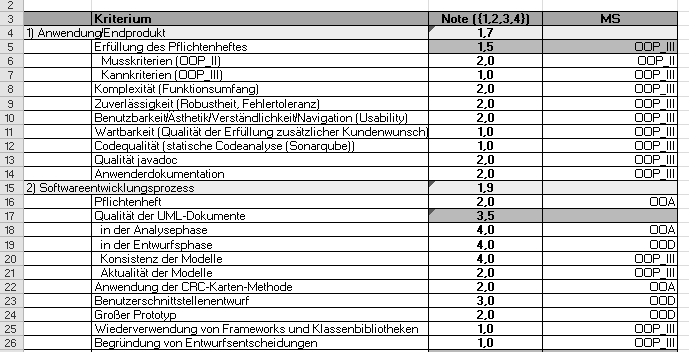
\includegraphics [width=\textwidth] {bewertung.png}
					\caption{Abschnitt der Bewertungstabelle für die Softwarepraktikumsgruppen}
					\label{bewertung}
				\end{figure}
  			\subsection{Selbsteinschätzung der Gruppen}
  				Die Selbsteinschätzung der Gruppen liegt in Form ausgefüllter Fragebögen vor, die die Gruppen nach erfolgreichem Abschluss des Softwarepraktikums ausfüllen. Im Gegensatz zu den Teilnoten der Tutorenbewertung sind hierbei allerdings nicht alle Angaben zur Verwendung in der angestrebten Analyse geeignet. In erster Linie fallen alle textuellen Beurteilungen und Kommentare heraus, da hier keine standardisierte Ermittlung der Zusammenhänge erfolgen kann. Darüber hinaus wurden auch die meisten Ja-Nein-Fragen nicht betrachtet, da diese keine aufschlussreichen Ergebnisse erwarten lassen und die zu analysierenden Daten nur unnötig erweitern würden. In Tabelle~\ref{survey} sind die ausgewählten Fragen aus den Fragebögen und die Art der jeweiligen Daten aufgelistet. Die textuell beschriebenen Skalen bei einem Teil der Fragen wurden in einfache numerische Skalen übertragen. Durch die vorgenommenen Einschränkungen wurden lediglich weitere 13 Vergleichsdatenreihen der Excel-Tabelle hinzugefügt.
  				\begin{center}
					\tabulinesep=1.5mm
					\begin{longtabu}{|p{0.4\textwidth}|p{0.5\textwidth}|}
						\hline
  						\textbf{Fragestellung} & \textbf{Datenbereich} \\
  						\hline
    					Anteil des Einarbeitungsaufwands am Gesamtaufwand & 0 bis 100 Prozent\\
    					\hline
    					Durchschnittlicher Arbeitsaufwand pro Woche und Student & Numerisch, in Stunden\\
    					\hline
    					Gleichverteilung des Aufwands & Ja (1) / Nein (0)\\
    					\hline
    					Bewertung Praktikumsergebnisses & "`Gerade so erfüllt"' (1) bis "`Übererfüllt"' (5)\\
    					\hline
    					Qualität der Analyse & "`Gerade so erfüllt"' (1) bis "`Übererfüllt"' (5)\\
    					\hline
    					Qualität des Entwurfs & "`Gerade so erfüllt"' (1) bis "`Übererfüllt"' (5)\\
    					\hline
    					Qualität von Implementation und Test & "`Gerade so erfüllt"' (1) bis "`Übererfüllt"' (5)\\
    					\hline
    					Qualität der Dokumentation & "`Gerade so erfüllt"' (1) bis "`Übererfüllt"' (5)\\
    					\hline
    					Anwendung der CRC-Methode & Hilfreich (1) / Nicht Hilfreich (0)\\
    					\hline
    					Das SalesPoint-Framework war eine Hile bei der Lösung der Aufgabe & Ja (1) / Nein (0)\\
    					\hline
    					Konsistenz zwischen Modellen und Code hergestellt & Gar Nicht (0) bis Sehr Stark (10)\\
    					\hline
    					Auf Konsistenz zwischen Modellen und Code geachtet & Gar Nicht (0) bis Sehr Stark (10)\\
    					\hline
    					Testfälle aus Modellen abgeleitet & Gar Nicht (0) bis Sehr Stark (10)\\
    					\hline
    					\caption{Für die Analyse ausgewählte Fragen der Selbsteinschätzung durch die Praktikumsgruppen. Die Werte in Klammern entsprechen der abgeleiteten numerischen Skala}
						\label{survey} \\
  					\end{longtabu}  
  				\end{center}

  	\chapter{Analyse der Messergebnisse}
  		Nach erfolgter Vermessung aller zur Verfügung stehender Programme, sowie der Aufbereitung der Messergebnisse und Vergleichswerte in Form einer Excel-Tabelle, galt es nun, die Datenreihen zu Vergleichen und Zusammenhänge zu identifizieren. Im Folgenden soll das Konzept und die Durchführung für diese Analyse kurz vorgestellt werden, bevor auf die abgeleiteten Ergebnisse näher eingegangen wird.
  		\section{Konzept und Durchführung}
  			\subsection{Berechnung der Korrelation}
  				Zusammenhänge zwischen Datenreihen werden üblicherweise mittels der Berechnung des Korrelationskoeffizienten nach Bravais-Pearson ($r$) ermittelt \cite{Korrelation}. Dieser gibt den Grad der linearen Abhängigkeit an. Die Berechnungsvorschrift dazu sieht folgendermaßen aus:
  				\begin{equation}
					\Large{r = \dfrac{\sum_{i=1}^{n}(x_i - \bar{x})(y_i - \bar{y})}{\sqrt{\sum_{i=1}^{n}(x_i - \bar{x})^2} * \sqrt{\sum_{i=1}^{n}(y_i - \bar{y})^2}}}
				\end{equation}
				Dabei gilt 
				\begin{itemize}
					\item $n =$ Anzahl der Elemente je Datenreihe
					\item $x_1,... ,x_n =$ Die Elemente der ersten Datenreihe
					\item $y_1,... ,y_n =$ Die Elemente der zweiten Datenreihe
					\item $\bar{x} = \dfrac{1}{n} * \sum_{i=1}^{n}x^i$ (arithmetisches Mittel der ersten Datenreihe)
					\item $\bar{y} = \dfrac{1}{n} * \sum_{i=1}^{n}y^i$ (arithmetisches Mittel der zweiten Datenreihe)
				\end{itemize}
				Das Resultat der Berechnung ist ein Wert zwischen $-1$ und $1$. Bei $r=0$ gilt, dass die Datenreihen stochastisch unabhängig voneinander sind, es also keinen Zusammenhang gibt. Bei $r=1$ liegt ein positiver linearer Zusammenhang vor und bei $r=-1$ ein negativer linearer Zusammenhang. Die Zusammenhänge werden sichtbar, wenn man die Datenreihen in einem zweidimensionalen Koordinatensystem einträgt (siehe Abbildung~\ref{sample}). \newline
				\begin{figure} [h]
					\centering
					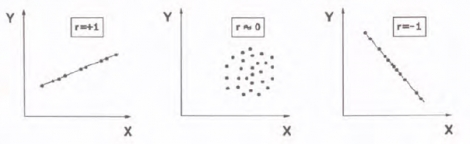
\includegraphics [width=0.7\textwidth] {sample.jpg}
					\caption{Beispielhafte Darstellung verschiedener Korrelationen im zweidimensionalen Koordinatensystem \cite{WasKorrel}}
					\label{sample}
				\end{figure}
				Die Berechnung der Korrelation übernimmt Excel mit der Formel $KORREL(Matrix1;Matrix2)$ \cite{ExcelKorrel}. Ohne diese automatische Berechnung wäre eine Gegenüberstellung dieser Datenmengen nicht möglich gewesen. Auf diese Art wurden also den 51 Messwerten und Metrikergebnissen 65 Bewertungen und Selbsteinschätzungen für jeweils 48 Gruppen ( $=$ Datenreihengröße $n$) gegenübergestellt und somit 3315 Korrelationskoeffizienten ermittelt. Die Ergebnisse erstrecken sich (unabhängig vom Vorzeichen) von 0,0000128, was sehr nah an stochastischer Zufallsverteilung liegt, bis hin zu 0,5533, was einen Zusammenhang vermuten lässt. Um aus den ermittelten Korrelationskoeffizienten Aussagen abzuleiten sind allerdings weitere Berechnungen notwendig.
			\subsection{Signifikanzermittlung}
				Um zu Entscheiden, ob eine ermittelte Korrelation Aussagekräftig ist bietet sich die Berechnung des p-Werts, also der Signifikanz an \cite{Signifikanz}. Dieser gibt an, wie wahrscheinlich eine ermittelte Korrelation zufällig zustande gekommen ist, und hängt von der Größe der Datenreihen ab. Je geringer diese Wahrscheinlichkeit ist, desto signifikanter ist die Korrelation. Üblicherweise werden folgende Signifikanzniveaus verwendet:
				\begin{itemize}
					\item Bei $p < 0,05$: signifikantes Ergebnis
					\item Bei $p < 0,01$: sehr signifikantes Ergebnis
					\item Bei $p < 0,001$: hoch signifikantes Ergebnis
				\end{itemize}
				Zur Berechnung der p-Werte wurde ein Online-Rechner verwendet \cite{PValue}. Für die verwendete Datenreihengröße von 48 Elementen ergeben sich damit folgende Grenzwerte für die ermittelten Korrelationskoeffizienten:
				\begin{itemize}
					\item Signifikant bei $r>=0,29$
					\item Sehr Signifikant bei $r>=0,37$
					\item Hoch Signifikant bei $r>=0,47$
				\end{itemize}
				In der Tabelle mit den ermittelten Korrelationen wurden daher alle Ergebnisse farblich markiert die diese Niveaus überschreiten. Alle anderen Gegenüberstellungen von Bewertung und Metrik werden als nicht zusammenhängend betrachtet. Das Niveau "`Hoch Signifikant"' wurde dabei nur bei zwei Metriken und sechs Messwerten überhaupt erreicht. \newline
				Die damit entstandene Korrelationstabelle, mit den Markierungen für als signifikant erkannte Einträge, bildet die Grundlage für die Ableitung von Aussagen bezüglich der Aussagekraft von Metriken und der damit verbundenen Verwendbarkeit des entstandenen PlugIns als teilautomatisiertes Bewertungssystem. 
				\newpage
  		\section{Ergebnisse} \label{Analyseergebnisse}
  			\subsection{Durchschnittsmetriken}
  				Die erste Auffälligkeit besteht darin, dass die ermittelten Durchschnittswerte für Qualität und Komplexität der Programme keine einzige, zumindest sehr signifikante Korrelation zu einer Bewertung aufweisen. Lediglich vereinzelte signifikante Werte bei wenigen Teilnoten und Selbsteinschätzungen treten auf. Auf diese sollte aber Aufgrund der im Endprodukt berechneten Werte keine Rückschlüsse getroffen werden können. Dies sind im einzelnen:
  				\begin{itemize}
  					\item Wie sehr wurde auf die Konsistenz der UML-Modelle geachtet?
  					\item Wie schätzen sie die Qualität des Entwurfs ein?
  					\item Bewertung Pflichtenheft
  					\item Bewertung Qualität der UML-Modelle im Entwurf 
				\end{itemize}  
				Hinzu kommt, dass der Zusammenhang entgegen der Erwartung verläuft. Je besser die Bewertung beziehungsweise Selbsteinschätzung ausfiel, desto komplexer und qualitativ schlechter wurden die Programme von den Metriken bewertet.	\newline
				Diese als Endergebnisse der Vermessung und Berechnung geplanten Metriken eignen sich also definitiv nicht zur Bewertung der Gruppen.			  
  			\subsection{Code-Quality-Index}
  				Ebenso ungeeignet zur teilautomatisierten Bewertung ist die umgesetzte Variante des Code-Quality-Index. Die einzige, gerade so signifikante Korrelation besteht zur Teilnote "`Erfüllung des Kundenwunsches"' der Projektphase III. Ob das Konzept grundsätzlich falsch ist, die vorgenommenen Anpassungen das Problem sind oder die Auswahl der Regeln für die Indikatoren die Ursache hierfür sind lässt sich aus den durchgeführten Messungen nicht ableiten. Dafür wäre eine variable Umsetzung mit verschiedenen Stellschrauben notwendig, um Vergleichsmessungen diverser Varianten durchzuführen.
  			\subsection{Zusammenhang zur Bewertung der Code-Qualität}
  				Aus Sicht der Teilnoten wäre besonders interessant, ob es einige Metriken gibt, die eine hohe Korrelation zur Bewertung der Code-Qualität aufweisen. Allerdings hat sich auch diese Erwartung nicht bestätigt. Lediglich die Qualitätsmetrik "`Conformity"' weißt einen signifikanten Zusammenhang zu dieser Teilnote auf. Die von den Tutoren wahrgenommene Code-Qualität spiegelt sich also im wesentlichen nicht in den von Harry Sneed vorgeschlagenen Metriken wieder. Auch dies bedeutet nicht zwangsläufig, dass die Metriken vom Konzept her ungeeignet sind, um Codequalität zu bewerten. Durch die Adaption in SonarQube, die abweichende Messwerte erzeugt und damit zum Teil auch Anpassungen der Metriken erforderte, wäre es durchaus möglich, dass das Ergebnis lediglich verfälscht wurde. Außerdem besteht die Möglichkeit, dass die Metriken lediglich für den Kontext des Softwarepraktikums ungeeignet sind. Herr Sneed setzt diese Metriken schließlich seit vielen Jahren erfolgreich in seiner Arbeit mit deutlich größeren Projekten in der Wirtschaft ein.
			\subsection{Konformität}  	
				Die bezüglich der Bewertung der Code-Qualität signifikant korrelierende Metrik "`Conformity"' ist generell die einzige Metrik die in diesem Kontext, mit dieser Umsetzung gute Ergebnisse erzielt. Die Metrik berechnet sich als, gemäß der Einstufung der Regeln, gewichtete Summe der Regelverletzungen, normiert durch die Anzahl der Anweisungen als Maß für die Größe des Programms (siehe Kapitel~\ref{messungchapter}).	Aufgrund der Masse an 	signifikanten Korrelationen, die zum Teil auch als "`sehr"' oder "`hoch"' signifikant eingestuft werden (siehe Tabelle~\ref{conformitykorrel}), lassen sich einige Erkenntnisse ableiten:
				\begin{itemize}
					\item Das zusammengestellte Regelwerk ist zumindest ein Schritt in die richtige Richtung und eignet sich für den Einsatz im Softwarepraktikum. Gruppen die weniger Regelverletzungen im Code haben, gemessen an der Größe des Programms, wurden hinsichtlich des Programms in vielen Teilnoten tendenziell besser bewertet. Dies gilt sogar, obwohl das Regelwerk weder den Gruppen, noch den Tutoren vorlag. 
					\item Je weniger Regelverletzungen im Programm enthalten sind, desto besser fällt auch die Selbsteinschätzung der Gruppen bezüglich der Qualität von Implementation und Test aus. An dieser stelle stimmen also alle drei Sichten auf die Qualität des Programms tendenziell überein.
					\item Da auch diverse Teilnoten bezüglich des Entwicklungsprozesses signifikant korrelieren lässt sich darüber hinaus sagen, dass bei denjenigen Gruppen die diese Regeln vermehrt einhalten auch der Test und die Projektphase III tendenziell besser ausfallen.
					\item Da im Gegensatz zur Metrik die reine Menge der verschiedenen Regelverletzungen deutlich weniger Korrelationen aufweisen, ist die Art der Aggregation sinnvoll gewählt und eine echte Bereicherung zu den Standard-SonarQube-Funktionen.
				\end{itemize}
				\begin{center}
					\tabulinesep=1.5mm
					\begin{longtabu}{|p{0.5\textwidth}|c|p{0.25\textwidth}|}
						\hline
  						\textbf{Bewertungspunkt / Einschätzung} & \textbf{Korrelation} & \textbf{Signifikanzniveau}\\
  						\hline
    					Anwendung / Endprodukt & -0,54063517 & hoch signifikant \\
    					\hline
						Erfüllung des Pflichtenheftes & -0,326289193 & signifikant \\
						\hline
						Musskriterien (OOP II) & -0,314500712 & signifikant \\
						\hline
						Komplexität (Funktionsumfang) & -0,472332933 & hoch signifikant \\
						\hline
						Zuverlässigkeit (Robustheit, Fehlertoleranz) & -0,417102682 & sehr signifikant \\
						\hline
						Wartbarkeit (Qualität der Erfüllung zusätzlicher Kundenwunsch) & -0,369214466 & signifikant \\
						\hline
						Codequalität (statische Codeanalyse (Sonarqube)) & -0,354376765 & signifikant \\
						\hline
						Qualität javadoc & -0,532658836 & hoch signifikant \\
						\hline
						Softwareentwicklungsprozess & -0,38982858 & sehr signifikant \\
						\hline
						Wiederverwendung von Frameworks und Klassenbibliotheken & -0,297004078 & signifikant \\
						\hline
						Qualität des Testens & -0,457170403 & sehr signifikant \\
						\hline
						junit-Tests durch die einzelnen Entwickler & -0,410540573 & sehr signifikant \\
						\hline
						Testabdeckung & -0,522114216 & hoch signifikant \\
						\hline
						OOP III & -0,385356884 & sehr signifikant \\
						\hline
						Stabilisierung der Anwendung & -0,298514637 & signifikant \\
						\hline
						Erfüllung des Kundenwunsches & -0,372836725 & sehr signifikant \\
						\hline
						AP Diskussion/Reaktion auf Fragen & -0,303573323 & signifikant \\
						\hline
						Note & -0,355579568 & signifikant \\
						\hline
						 Wie schätzen Sie die Qualität folgender Teilergebnisse ein? Implementation und Test & 0,344601363 & signifikant \\
    					\hline
    					\caption{Signifikante Korrelationen der Conformity-Metrik zu Tutorenbewertungen und Selbsteinschätzungen der Gruppen}
						\label{conformitykorrel} \\
  					\end{longtabu}  
  				\end{center}
  			\subsection{Datenflusskomplexität}
  				Neben der Conformity-Metrik gibt es noch eine Weitere, die auffällig viele signifikante Korrelationen zu Teilnoten aufweist. Dabei handelt es sich um die "`Data-Flow-Complexity"' die letztlich das Verhältnis zwischen Variablendeklarationen und Variablenreferenzen darstellt (siehe Kapitel~\ref{messungchapter}). Werden wenige Variablen oft referenziert, spricht dies laut Sneed für eine hohe Komplexität im Programm \cite{SoftwareInZahlen}, was wiederum eine schlechtere Bewertung zur Folge haben sollte. Der ermittelte Zusammenhang verhält sich allerdings genau anders herum. Nach dieser Metrik komplexere Programme werden tendenziell besser bewertet. In diesem Kontext, mit dieser Umsetzung ist die Metrik also vom Ansatz her vollkommen falsch und damit unverwendbar. Warum gerade diejenigen Programme besser bewertet wurden, die im Verhältnis zu den Variablendeklarationen besonders viele Variablenreferenzen enthalten, müsste separat untersucht werden.
  			\subsection{Größe der Projekte}
  				Es gibt eine ganze Reihe signifikanter Korrelationen diverser Messwerte zu einigen der Teilnoten. Da die Messwerte im wesentlichen nur ein Spiegel der Größe des vermessenen Programms sind und die Werte für Netto-Code-Zeilen und Object-Points ebenfalls einige solcher Korrelationen aufweisen, lässt sich daraus ableiten, dass die umfangreicheren der abgelieferten Programme tendenziell auch die besseren sind. Dieser Zusammenhang eignet sich aber nicht zur teilautomatisierten Bewertung, da ein größeres Programm eben gerade nicht automatisch gut ist. Aufgrund der geringen Bedeutung dieses Zusammenhangs wird daher auf eine Auflistung der konkreten Korrelationen verzichtet. Besonders Gehäuft treten signifikante Zusammenhänge bei den Teilnoten für das Programm, die UML-Dokumente, den Test, die Projektphase III sowie die Abschlusspräsentation auf.
  			\subsection{Projektmanagement und Teamarbeit}
  				Auffällig Aufgrund beinahe nicht vorhandener signifikanter Korrelationen ist darüber hinaus die Bewertung des Projektmanagements und der Teamarbeit. Sämtliche Teilnoten dieser Bereiche weisen nahezu keine signifikanten Korrelationen zu Messwerten und als relevant eingestuften Metriken auf. Die Organisation der Teams untereinander scheint also einen recht geringen Einfluss auf das zu entwickelnde Programm und den Entwicklungsprozess zu haben.
  			\subsection{Vereinzelte signifikante Korrelationen}
  				Neben den genannten Auffälligkeiten aus denen sich Rückschlüsse ableiten lassen tauchen vereinzelt signifikante bis hoch signifikante Korrelationen in den Daten auf, die sich nicht sinnvoll begründen lassen. Dazu zählt beispielsweise, dass Gruppen die angeben, dass der Arbeitsaufwand nicht gleich verteilt war, tendenziell mehr numerische Literale im Code verwenden (Korrelation -0,484926924). Ähnlich signifikant ist der Umstand, dass Gruppen die angeben wenig auf die Konsistenz der UML-Modelle zu achten besonders viele Regeln der Kategorie "`minor"' verletzen (Korrelation -0,496352551). Für sich allein gestellt ist auch die höchste ermittelte Korrelation von -0,553331812 wenig aufschlussreich. Gruppen, die bezüglich der Diskussionsrunde bei der Abschlusspräsentation gut bewertet wurden, haben in ihren Programmen tendenziell mehr private Methoden deklariert. Diesen möglicherweise zufälligen, vielleicht aber auch systematischen Zusammenhängen wird im Rahmen dieser Arbeit keine weitere Aufmerksamkeit geschenkt, da es unwahrscheinlich ist, dass sich daraus eine praktische Verwendbarkeit für das Softwarepraktikum ergibt.
  		\section{Einschränkungen}
  			Die abgeleiteten Erkenntnisse unterliegen einer ganzen Reihe von Beschränkungen und sind damit weit entfernt von Allgemeingültigkeit oder Unanfechtbarkeit. Im Folgenden sollen die Bedeutendsten kurz genannt und erläutert werden.
  			\begin{labeling}{\textbf{Stichprobengröße}}
				\item [\textbf{Vergleichswerte}] Die Analyse geht davon aus, dass die zum Vergleich herangezogene Bewertung der Gruppen objektiv, korrekt und einheitlich ist. Da die Teilnehmer allerdings von vielen verschiedenen Tutoren mit ganz unterschiedlichen Erfahrungen und Wissensständen bewertet werden kann dies offensichtlich nicht vollständig zutreffen. Allein die persönliche Auswahl der Programmierregeln die als notwendig für gute Code-Qualität erachtet wird kann stark variieren. Dies zeigt sich in der Auswertung der untersuchten Regelwerke eindrucksvoll (siehe Kapitel~\ref{regelwerke}). Diese sind ebenfalls sehr unterschiedlich und zum Teil widersprechen sich die enthaltenen Regeln sogar. Es ist daher davon auszugehen, dass die Maßstäbe zur Bewertung die von den einzelnen Tutoren angesetzt werden, trotz entsprechender Richtlinien vom Lehrstuhl, voneinander abweichen können. Eine bessere Beurteilung der Metrikergebnisse könnte erreicht werden, wenn als Vergleichsgröße eine einheitliche Bewertung aller Gruppen durch einen Experten, beziehungsweise eine kleine Gruppe von Experten herangezogen würde.
				\item [\textbf{Stichprobengröße}] Trotz der Vermessung von zwei kompletten Jahrgängen ist die resultierende Stichprobe mit 48 untersuchten Gruppen noch relativ klein. Mit einer noch umfangreicheren Vermessung ließen sich die Ergebnisse verbessern. Dies würde auch durch subjektive Bewertung entstandene Verzerrung abmildern.
				\item [\textbf{Methodik}] Die bei der Analyse verwendete Methode der Korrelationsberechnung und Signifikanzbeurteilung mittels p-Wert lässt nur bedingt Rückschlüsse zu. Im Grunde liefert sie nur Hinweise auf scheinbar linear zusammenhängende Sachverhalte. Ob dieser Zusammenhang tatsächlich besteht oder doch ein Zufall vorliegt lässt sich nicht belegen. Auch die Möglichkeit nicht-linearer Zusammenhänge wurde nicht betrachtet. Insbesondere lassen sich aber aus signifikanten Korrelationen keine Kausalitäten ableiten. Es bleibt also für zukünftige Arbeiten zu prüfen, ob die Einführung des erstellten Regelwerks und eine vermehrte Einhaltung dieser Regeln tatsächlich zu besserer Code-Qualität führen.
				\item [\textbf{Kontext}] Die getroffenen Aussagen sind wie bereits erwähnt ausschließlich im Kontext des Softwarepraktikums zu sehen. Sie gelten also nur für kleine Java-Programme mit dem SalesPoint-Framework, die von kleinen Gruppen relativ unerfahrener Studenten im Rahmen dieser Lehrveranstaltung implementiert werden. Eine Übertragung auf größere Projekte, erfahrene Entwickler, andere Programmiersprachen oder auch private studentische Projekte ist nicht möglich.
			\end{labeling}
  	\chapter{Zusammenfassung und Ausblick}
  		Seit den ersten Ideen für Metriken zur Bewertung der Qualität und Komplexität einer Software stehen diese auch in der Kritik. Es konnte nie erschöpfend nachgewiesen werden, dass es eine Metrik gibt, die sich dafür wirklich gut eignet. So beschreibt Martin Shepperd bereits 1988 in seiner Kritik an McCabes zyklomatischer Komplexität, dass deren Zusammenhang mit der Wartbarkeit und Testbarkeit einer Software nicht größer ist, als der Zusammenhang zwischen diesen Merkmalen und der simplen Softwaregröße in Codezeilen \cite{McCabeCritique}. \newline
  		Auch spätere umfangreichere Untersuchungen verschiedenster Metriken konnten keine Metrik identifizieren, deren Korrelation zu einer Qualitätseigenschaft des Codes signifikant größer ist als die Korrelation zwischen dieser Eigenschaft und der Größe des Codes. Yossi Gil and Gal Lalouche kommen daher zu dem Schluss, dass die Größe einer Software die einzige valide Codemetrik ist \cite{SizeOnlyMetric}. \newline
  		Es ist daher wenig überraschend, dass es auch im Rahmen dieser Arbeit nicht gelungen ist eine Menge von Codemetriken zu finden mit denen sich die Codequalität automatisiert bewerten lässt. Mit dem Regelwerk und der darauf aufbauenden Conformity-Metrik ließ sich trotzdem ein verwendbarer Gewinn für zukünftige Softwarepraktika erreichen. Der Satz von Horst Zuse mit dem der vorangegangene Große Beleg eingeleitet wurde bleibt aber bestehen \cite{FrameworkSoftwareMeasurement}:
  		\begin{quote}
  			"`One number can not express softwarequality!"'
  		\end{quote} 
  		\section{Beantwortung der Forschungsfragen}
			Abschließend lässt sich also feststellen, dass das Ziel eines teilautomatisierten Bewertungssystems nicht erreicht wurde. Keine der umgesetzten Metriken oder Kennzahlen bietet genug Aussagekraft um dies umzusetzen. Trotzdem sollen die Anfangs formulierten Forschungsfragen an dieser Stelle kurz zusammenfassend beantwortet werden.
			\begin{itemize}
				\item \textbf{Nach welchen Programmierregeln sollte die Bewertung hinsichtlich Codequalität im Kontext des Softwarepraktikums erfolgen?} \newline \newline
				Das Regelwerk wurde auf Basis vielfältiger Recherche zusammengestellt und hat sich in der Analyse als gute Basis für zukünftige Softwarepraktika herausgestellt (siehe Tabelle~\ref{ruleset}). Trotzdem sollte es nicht als feste Größe betrachtet werden. Im Verlauf der nächsten Jahrgänge sollte kontinuierlich überprüft werden ob die Regeln noch sinnvoll sind, oder ob es notwendig ist Regeln zu streichen, ersetzen, ändern oder hinzuzufügen. Auch zukünftige Neuerungen in Java oder dem SalesPoint-Framework könnten Änderungen notwendig machen.
				\item \textbf{Inwiefern ist eine Umsetzung des Code-Quality-Index in SonarQube möglich und welche Anpassungen sind notwendig oder sinnvoll?} \newline \newline
				Während der Konzeption des Code-Quality-Index ergaben sich diverse Anpassungen, die zum Teil auch notwendig waren um den Index überhaupt umsetzen zu können. In der abschließenden Analyse hat sich allerdings herausgestellt, dass der Index in dieser Form nicht funktioniert. Es erscheint wahrscheinlich, dass der Code-Quality-Index sich zurecht nicht als Werkzeug zur Beurteilung von Code-Qualität durchgesetzt hat und als gescheitert zu betrachten ist. Es ist aber ebenso vorstellbar, dass mit geeigneteren Anpassungen eine praktikable Variante gefunden werden kann. Um dies zu evaluieren wäre allerdings eine Implementierung notwendig, die es erlaubt viele Parameter zu konfigurieren um so diverse Messreihen zu erzeugen die miteinander verglichen werden können.
				\item \textbf{Lässt sich die Stabilität und Wartbarkeit des PlugIns durch die Verwendung von ExtendJ/Jastadd verbessern?} \newline \newline
				Die Wartbarkeit des PlugIns lies sich durch den Einsatz von ExtendJ massiv verbessern und auch der Entwicklungsaufwand wurde deutlich reduziert. Die Einarbeitung in die Attributdefinition ist ohne weiteres im Rahmen einer Diplomarbeit möglich. Allerdings führen einige Fehler in JastAdd dazu, dass ein Teil der Praktikumsprojekte nicht vermessen werden kann. Da sich das PlugIn als nicht einsetzbar erwiesen hat wurde allerdings auch keine weiterführende Fehleranalyse und Korrektur versucht. Dies wäre notwendig um ein PlugIn auf der Basis des ExtendJ-Parsers für das Softwarepraktikum einzusetzen.
				\item \textbf{Welche Methoden eignen sich, um die Aussagekraft der Metriken zu evaluieren?} \newline \newline
				Mit der angewendeten Methode der Korrelationsermittlung und Signifikanzbeurteilung mittels p-Wert ließen sich einige Erkenntnisse über die umgesetzten Metriken gewinnen. Eventuell wären weiterführende Analysen sinnvoll um die Resultate zu untermauern.
				\item \textbf{Welche der umgesetzten Metriken und Bewertungssysteme eignen sich zur teilautomatisierten Bewertung zukünftiger Softwarepraktika?} \newline \newline
				Keine der untersuchten Metriken eignet sich dafür hinreichend. Allerdings scheint das erstellte Regelwerk in Verbindung mit der "`Conformity"'-Metrik ein guter Indikator für Code-Qualität zu sein, die insgesamt zu einem besseren Programm führt.
			\end{itemize}
		\section{Verwendungsmöglichkeiten der Implementierung}
			Die Implementierung, die zur Vermessung der letzten beiden Jahrgänge verwendet wurde ist nicht für den produktiven Einsatz bei zukünftigen Softwarepraktika geeignet. Dies hat folgende Ursachen:
			\begin{itemize}
				\item Fehler im Parser: Manche Programme können nicht vermessen werden.
				\item Viele Zahlen ohne Bedeutung: Die Metriken würden mehr Verwirrung stiften, als helfen, da sie zumeist keinen Hinweis auf die tatsächliche Qualität liefern.
				\item Fehlende GUI: Aufgrund der Analyseergebnisse wurde auf eine Umsetzung verzichtet.
			\end{itemize}
			Sie könnte allerdings für zukünftige Arbeiten als Basis dienen. Das PlugIn enthält eine große Anzahl von Messwerten die zur Evaluierung anderer Metriken wiederverwendet werden könnten. Auch eine Überarbeitung der Indeximplementation ist denkbar. \newline
			Für den produktiven Einsatz im Softwarepraktikum wurde stattdessen ein Mini-PlugIn erstellt, dass lediglich die "`Conformity"'-Metrik und eine Abwandlung der Object-Points berechnet. Dieses PlugIn kommt ohne den Parser aus, da nur Standard-SonarQube-Messwerte verwendet werden. Somit entfällt die Fehleranfälligkeit. Auch die zusätzlichen Datenbankschemata sind für dieses PlugIn nicht notwendig. Damit reduziert sich auch die Ausführungszeit deutlich. Die zwei berechneten Metriken werden in einem simplen Widget angezeigt und können so die Tutoren bei der Bewertung der Code-Qualität unterstützen. Auf eine manuelle Analyse der Regelverletzungen im Detail kann weitestgehend verzichtet werden. Das Regelwerk ist ohnehin PlugIn-Unabhängig und kann über die Web-Oberfläche integriert werden. Darüber hinaus kann es den Studenten zur Verfügung gestellt werden und über entsprechende Erweiterungen auch in gängige IDEs wie Eclipse und IntelliJ eingebunden werden.
		\section{Weiterführende Fragestellungen}
			Wie teilweise bereits erwähnt bleiben viele Fragen und Möglichkeiten zur teilautomatisierten Bewertung der Codequalität offen. Im Folgenden einige Fragen, die man in weiterführenden Arbeiten untersuchen könnte:
			\begin{itemize}
				\item Inwiefern unterscheiden sich die Metrikergebnisse wenn die Berechnung mit SoftAudit vorgenommen wird? Möglicherweise liefert diese Umsetzung bessere Ergebnisse und kann auf anderem Wege ohne Anpassung in SonarQube oder einem anderen System integriert werden.
				\item Gibt es andere Metriken zur Beurteilung der Codequalität die aussagekräftiger sind?
				\item Sind die hier vorgestellten Erkenntnisse für zukünftige Softwarepraktika ebenso gültig, oder wurden Fehler gemacht?
				\item Lässt sich das Regelwerk weiter optimieren? Welche Regeln sind überflüssig oder kontraproduktiv? Welche sollten hinzugefügt werden? Ist die Conformity-Metrik noch zu verbessern?
			\end{itemize}			 		
  		
  	\backmatter
  
  	\appendix
  	\bibliography{diplombib}
  
\end{document}
